\documentclass{article}

\usepackage{amsmath}
\usepackage{amsfonts}
\usepackage[left=3cm,right=3cm,top=2.5cm,bottom=2.5cm]{geometry}
\usepackage[sort&compress]{natbib}
\bibliographystyle{apalike}
\usepackage{soul}
\usepackage{url}
\usepackage{circuitikz}
\usepackage{amsthm}
\usepackage[backref=page]{hyperref}
\usepackage{titlesec}
\usepackage{tikz}
\usepackage{array}
\usepackage{caption}
\usepackage{cleveref}
\usepackage[acronym]{glossaries}
\usepackage{subcaption}
\usepackage{bbm}

\usetikzlibrary{arrows, positioning, arrows.meta}


\newcommand{\xd}{x_{dist}}
\newcommand{\yt}{y_{temp}}
\newcommand{\indep}{\perp \!\!\! \perp}
\newcommand{\refp}[1]{(\ref{#1})}
\newcommand{\degrees}{$^{\circ}$}
\newcommand{\R}{\mathbb{R}}
\newcommand*\circled[1]{\tikz[baseline=(char.base)]{
            \node[shape=circle,draw,inner sep=2pt] (char) {#1};}}

\newtheorem{theorem}{Theorem}
\newtheorem{definition}{Definition}
\newtheorem{corollary}{Corollary}


\title{Active Inference}
\author{Jack Montgomery}
\date{July 2024}

\begin{document}

\begin{titlepage}
    \centering
    \vspace*{1in}
    
    {\LARGE \textbf{Communication in Multi-Agent Reinforcement Learning}}\\[2cm]
    
    {\large \textbf{Jack Montgomery}}\\[0.5cm]
    {\large MNTJAC003}\\[0.5cm]
    {\large MAM4000W - Advanced Topics in Reinforcement Learning}\\ [0.5cm]
    {\large University of Cape Town}\\[2cm]
    
    
\includegraphics[width=0.3\textwidth]{images/UCT_logo_circular_blue_large.png}\\[0.8cm]
    
    {\large November 2024}\\[1.4cm]
    
    \begin{abstract}
    Multi-agent reinforcement learning (MARL) is a growing field within artificial intelligence that presents challenges such as credit assignment, scalability, and non-stationarity. Reinforcement learning has close ties to theories of the dopamine system and classical conditioning. Moreover, `deep' reinforcement learning has been pioneered by the use of the multi-layer perceptron as a function approximator, which itself is motivated by the structure of neurons in the brain. This suggests that solutions to issues in multi-agent systems may benefit from mechanisms humans naturally employ - chiefly, communication. In this report, we establish foundational concepts in single-agent reinforcement learning, introduce core MARL theories, and explore how communication is implemented in the field. Lastly, we analyse the assumption of parameter sharing, a prevalent approach in contemporary MARL models.
    \end{abstract}
    
\end{titlepage}

\newpage

\tableofcontents

\newpage

\section{Introduction}

Many real world problems can be modelled as multi-agent systems, these include autonomous-driving \citep{shavlev2016safe}, sensor networks \citep{vinyals2014sensor} and robotics \citep{kober2013reinforcement}. The number of systems that can be modelled in this way is only increasing in an age of ubiquitous computing power and the use of artificial intelligence agents. This begs the question of how can a collective of autonomous agents, each capable of making its own decision, interact in this shared environment in order to achieve the goal of the environment. These agents may be homogenous with shared goals, as in the case of a fleet of robots, where each agent only benefits if the collective benefits, or different, heterogeneous agents who benefit from the other agent's failing a task. If agents do not have an understanding of the dynamics of the environment, or how rewards will be generated from the environment, can they use the experience of historical interactions to then learn these features and maximise the rewards they receive. This type of behaviour is very difficult to achieve with other agents' taking actions that too effecting the environment causing non-stationarity in the dynamics, and making it more difficult for an agent to understanding what exactly caused the reward they are observing, which is the problem of credit assignment. Solving these problems and achieving these intelligent multi-agent systems is the vision of multi-agent reinforcement learning (MARL). \citep{albrecht2024marl}

\

MARL is an extension of single-agent reinforcement learning (RL) \citep{sutton2018reinforcement} meaning that the MARL aims to use the framework's for modelling environments, as well as the techniques for learning from RL and adjust them to better suit a situation with multiple agents. RL has laid the foundation for artificial agent's learning from experience in an environment, with no (or very little) prior information about the dynamics or reward structure. Many core ideas in reinforcement learning are inspired by phenomena in animal learning, psychology and neuroscience. \citep{subramanian2020psychological} What's more, modern approaches in RL use so called `deep' methods \citep{wang2024deep} in which neural networks are used in as function approximators for various components of a reinforcement learning model. With neural networks too being inspired from the manner in which we understand our brain to be performing computations. The human experience has been fundamental to the development of these algorithms and solution techniques, it is therefore reasonable to consider how human's solve problems with many people as motivation for the approach to take in MARL. A fundamental mechanism for coordinating the behaviours of multiple agents, broadening their views of the environment, and to support their collaborations is \textbf{communication}. \citep{zhu2024survey}

\

Investigating how this communication can be realised within MARL is done in the subfield of multi-agent reinforcement learning with communication (Comm-MARL). Within Comm-MARL, we consider the structure of the communicative messages that are sent by agents, who the agent's are able to communicate with, how agent's learn to communicate, what kind of communication is encouraged by the environment etc.. Comm-MARL again builds on techniques from MARL with the addition of this dimension of communication and messages again needing to be incorporated into the frameworks and models. The goal of this report is to provide a thorough overview of the techniques of Comm-MARL, as well as investigate some of the common assumptions taken in Comm-MARL models. We aim to achieve this by placing reinforcement-learning building blocks on top of one another to ultimately land at the structure of Comm-MARL.

\

We will start this investigation with the foundations of RL in Section \ref{sec:rl}. We discuss the fundamental structural assumption of a system that can be solved using RL - the distinction of an environment and an agent. This structure then gives rise to the agent-environment loop for which learning algorithms aim to exploit in order to learn to solve the problem of the environment.  This distinction requires us to define two different sets of tools - frameworks for understanding the environment and models for maximising rewards. The framework for sequential decision problems we will be considering in this report are Markov decision processes (MDP). These sequential decisions processes carry an assumption of the dynamics of the states over time - that the chain of states of the environment has the \textbf{Markov property}. This assumption is used to construct algorithms to solve these decision problems. We will then move on to discuss the two types of models we will be considering - value-based and policy based. We will then build some intuition about these model categories by way of an example in a simple grid-world environment from OpenAI \textit{Gymnasium} \citep{kwiatkowski2024gymnasium} package. Finally, we will introduce the deep methods from RL that will then build the foundation for the multi-agent algorithms that are discussed later in the report.

\ 
 
We can then place the MARL building block with this intuition and understanding of RL; its environmental frameworks and models. The agent-environment loop nows becomes the agent\textbf{s}-environment loops in MARL. This requires a different set of environment frameworks to understand this problem. These tools build on MDPs and include multiple agent's, each of their local observations and the their reward structure. This is usually formalised as a partially observable stochastic game (POSG). Translating RL techniques fall on a spectrum between modelling all agents as a single agent with the joint observation and action space and assuming that agent's are independent actors and not considering the effect that other agent's have on the environment. These techniques, as well as other fundamental characteristics of multi-agent systems give rise to core problems of MARL which is discussed.


\

The final block we will place is communication on this MARL foundation. To overview this subfield we use the nine dimensions of Comm-MARL models identified in \citet{zhu2024survey} to compare and disambiguate five representative Comm-MARL algorithms: DIAL and RIAL \citep{foerster2016learning}, CommNet \citep{sukhbaatar2016commnet}, IC3Net \citep{singh2018ic3net}, BiCNet \citep{peng2017bicnet}, NeurComm \citep{chu2020NeurComm} and HAMMER \citep{gupta2022HAMMER}. The use of these models is to give concrete examples of the different approaches that have been taken to communication. While the neural network and training schemes are not introduced for each model in this report explicitly, we have included these details in Appendix \ref{sec:models}. That being said, reading through each dimension of Comm-MARL one will obtain a good overall understanding of these models. A point to note is that there is a particular approach to Comm-MARL that is called \textit{emergent language}. Although one can argue algorithms do not learn a language as humans know, this approach usually entails agents selecting a specific number of `words' from a predefined lexicon. The goal of the combination of these words is to resemble the descriptive and hierarchical nature of human language. This will not be addressed in this report, and we refer the reader to \citet{boldt2024review} for details of models and application of emergent language in machine learning.

\

The final section of this report will be a practical implementation of Comm-MARL. As we will see, parameter sharing is used extensively in Comm-MARL as it is a fundamental assumption for fully differentiable communication learning as well as allowing these algorithms to scale with the number of agents present. However, the practical implementation of parameter sharing is not feasible. \citep{terry2023revisiting} Since these methods do not allow for heterogeneous action or observations dimensions. Therefore in this final section we will compare a simple MARL learning algorithm with the presence and absence of communication and parameter sharing and discuss the implications thereof.

\

This report makes no attempt to present novel findings, but rather translate, condense and discuss the field of Comm-MARL. 

\newpage

\section{Reinforcement Learning (RL)} \label{sec:rl}

Reinforcement learning, much like machine learning, refers to both a problem as well as a class of solutions \citep{sutton2018reinforcement}. Reinforcement learning problems involve learning what to do - how to map situations to actions - so as to maximise a numerical reward signal. In an essential way they are closed-loop problems because the learning system’s actions influence its later inputs. Moreover, the learner is not told which actions to take, as in many forms of machine learning, but instead must discover which actions yield the most reward by trying them. In the most interesting and challenging cases, actions may affect not only the immediate reward but also the next situation and, through that, all subsequent rewards. These three characteristics - being a closed loop, not having direct instructions as to what actions to take, and where the consequences of actions, including reward signals, play out over extended time periods - are the three most important distinguishing features of reinforcement learning problems.


\subsection{Agent - Environment Loop}

Reinforcement learning is a framing of the problem of learning from interactions to achieve a goal. The decision maker (learner) is called the \textit{agent}. The thing it interacts with is called the \textit{environment}. These interact continually, the agent selecting actions and the environment responding to those actions and presenting new situations to the agent. The environment also gives rise to rewards. These are numerical values that the agent seeks to maximise over time.

\

Specifically, the agent and the environment interact over a sequence of discrete time-steps $(t = 1, 2, 3, \hdots)$ At each time-step the agent receives some representation of the environment's state, $S_t \in \mathcal{S}$ where $\mathcal{S}$ is the set of all possible states of the environment, based on that the agent selects an action, $A_t \in \mathcal{A}(S_t)$, where $\mathcal{A}(S_t)$ is the set of all possible actions the agent can take in state $s_t$. In the next time-step, the agent receives a numerical reward $R_{t+1} \in \mathcal{R} \subset \mathbb{R}$, and observes a new state representation $S_{t+1}$. This agent-environment loop is depicted in Figure \ref{fig:agent_environment}.

\

\begin{figure}
	\centering
	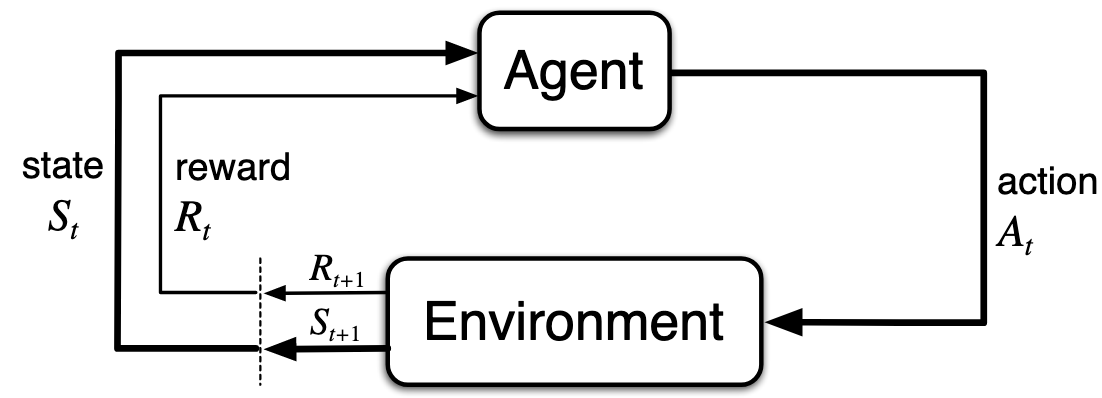
\includegraphics[scale=0.6]{images/agent_environment.png}
	\caption{Agent-environment loop from \citet{sutton2018reinforcement}}
	\label{fig:agent_environment}
\end{figure}

At each time-step the agent implements a mapping from states to a probability distribution over actions. The mapping is called the agent's \textit{policy} and is denoted $\pi_t(a | s)$ which represents the probability $A_t = a$ given $S_t = s$. This mapping fully characterises the agent's behaviour \citep{silver2015rl} so the goal of maximising the total amount of reward the agent receives becomes a problem of finding a policy that maximises the reward the agent receives. 

\subsection{Returns}

So far we have discussed the learning objective of reinforcement learning informally with the notion that the agent seeks to maximises the rewards it receives over time. Let us denote the sequence of rewards received after time $t$ as $R_{t+1}, R_{t+2}, R_{t+1} \hdots$, we cannot directly effect the reward signal after time $t+1$ from an action at time $t$. Therefore, we seek to maximise the \textit{expected return}, where the return $G_t$ is defined as some function of the rewards sequence. We make the assumption of discounting future rewards - meaning the agent has some bias towards rewards received sooner in the sequence. In particular, it chooses $A_t$ to maximise the \textit{expected discounted return}:

\begin{equation}\label{eq:returns}
	G_t = R_{t+1} + \gamma R_{t+2}+ \gamma^2 R_{t+3} + \hdots + \gamma^{T} R_{t+T+1} = \sum_{k=0}^T \gamma^k R_{t + k + 1}
\end{equation}

where $0 \leq \gamma \leq 1$ is called the \textit{discount factor}, and $T$ is the final time step.

\

Intuitively, a smaller value of $\gamma$ means the agent is more myopic. While a larger value means the agent will be more long-sighted in its selection of actions. This approach makes sense in applications in which there is a natural notion of final time step, that is, when the agent-environment interaction breaks naturally into subsequences, which we call \textit{episodes}.

\subsection{Markov Property}

 The state representation that the agent observes, $S_t$, forms a chain where $S_{t-1}$ is ``linked'' to $S_t$ through the action taken at time $t - 1$ ($A_{t-1}$). If this chain satisfies the \textit{Markov property} then the reinforcement learning task can be described as a \textit{Markov decision process} (MDP). The \textit{Markov property} means that all information that is needed by the agent can be found in its current state signal. The state signal should include immediate sensations such as sensory measurements, but it can contain much more than that. State representations can be highly processed versions of original sensations, or they can be complex structures built up over time from the sequence of sensations. For example, we can move our eyes over a scene, with only a tiny spot corresponding to the fovea visible in detail at any one time, yet build up a rich and detailed representation of a scene. \citep{sutton2018reinforcement}
 
 \
 
 The Markov property can be stated mathematically for the reinforcement learning problem by considering how an environment may response to an action at time $t$. In general, the reaction may depend on everything that has happened before:
 
 \begin{equation}
 	\mathbb{P}[ R_{t+1} = r, \ S_{t+1} = s' | S_0, A_0, \hdots, S_t, A_t]
 \end{equation}
 
 If we assume that chain of state signals does obey the Markov property, then the expression of the reaction of the environment can be simplified to:
 
 \begin{equation}
 	p(s', r | s, a) = \mathbb{P}[ R_{t+1} = r, \ S_{t+1} = s' | S_t, A_t]
 \end{equation}
 
 The Markov property is important in reinforcement learning because decisions and values are assumed to be a function only of the current state. In order for these to be effective and informative, the state representation must be informative. \citep{sutton2018reinforcement}

\subsection{Markov decision processes}

If the set of states and the set of actions are finite then the MDP is called a \textit{finite Markov decision process}. This is the foundational framework for reinforcement learning problems. 

\

A finite MDP is defined by its set of states $\mathcal{S}$, and the set of actions, $\mathcal{A}$. As well as by the one step dynamics of the environment. Given any state ($s \in \mathcal{S}$) and action ($a \in \mathcal{A}$) the probability of each possible pair of next states ($s' \in \mathcal{S}$) and reward ($r \in \mathcal{R}$) is denoted:

\begin{equation}
	p(s', r | s, a) = \mathbb{P}[ R_{t+1} = r, \ S_{t+1} = s' | S_t, A_t]
\end{equation}

These quantities fully define a finite MDP.

\subsection{Value Functions}

Almost all solutions to reinforcement learning problems involve some estimation of the ``goodness'' of states. Intuitively this makes sense as we need some understanding of the reward dynamics before we could hope to find a policy that maximises these rewards. The ``goodness'' is measured in terms of discounted expected future returns (\ref{eq:returns}) and is encapsulated in the \textit{value function}. Of course the rewards the agent can expect to receive in the future depend on what actions it will take. Accordingly, value functions are defined with respect to particular policies. Formally, the value function is expressed as:

\begin{equation}\label{eq:value_function}
	v_\pi(s) = \mathbb{E}_\pi\left[ G_t \middle| S_t = s \right] = \mathbb{E}_\pi\left[ \sum_{k=0}^T \gamma^t R_{t + k + 1} \middle| S_t = s \right]
\end{equation}

Similarly, we define the value of taking action $a$ in state $s$ under a policy $\pi$, denoted $q_\pi(s, a)$, as the expected return starting from $s$, taking the action $a$, and thereafter following policy $\pi$:

\begin{equation}
	q_\pi(s, a) = \mathbb{E}_\pi \left[ G_t  \middle| S_t = s, A_t = a\right] = \mathbb{E}_\pi \left[ \sum_{k=0}^T R_{t + k + 1} \middle| S_t = s, A_t = a\right]
\end{equation}

We will call $v_\pi$ the value of a state and the $q_\pi$ the q-value of a state-action pair.

\

The functions $v_\pi$ and $q_\pi$ can be estimated from experience. For example, if an agent follows policy $\pi$ and maintains an average, for each state encountered, of the actual returns that have followed that state, then the average will converge to the state’s value, $v_\pi(s)$, as the number of times that state is encountered approaches infinity. If separate averages are kept for each action taken in a state, then these averages will similarly converge to the action values, $q_\pi(s, a)$. These estimation techniques are called \textit{Monte Carlo methods} because they involve averaging over many random samples of actual returns. Of course, if there are very many states, then it may not be practical to keep separate averages for each state individually. Instead, the agent would have to maintain $v_\pi$ and/or $q_\pi$ as parameterised functions and adjust the parameters to better match the observed returns. This can also produce accurate estimates, although much depends on the nature of the parameterised function approximator. These methods will be covered in Section \ref{sec:deep_rl}.

\

A fundamental property of value functions used throughout reinforcement learning is that they satisfy particular recursive relationships. For any policy $\pi$ and any state $s$, the following consistency condition holds between the value of s and the value of its possible successor states:

\begin{equation}\label{eq:bellman_equation}
	v_\pi(s) = \mathbb{E}_\pi [ G_t | S_t = s ] = \sum_a \sum_{s', r} p(s', r | s, a) \left[ r + \gamma v_\pi(s') \right]
\end{equation}

This expression is known as the Bellman equation for $v_\pi$. It expresses a relationship between the value of a state and the values of its successor states. We will see that this expression forms the basis of a number of techniques to compute, approximate and learn $v_\pi$.

\subsection{Optimal Value Functions}

As mentioned, solving a reinforcement learning problem means finding a policy that maximises the rewards over time. For finite MDPs, we can precisely define an optimal policy in the following way. Value functions define a partial ordering over policies. A policy $\pi$ is defined to be better than or equal to a policy $\pi'$ if its expected return is greater than or equal to that of $\pi'$ for all states. In other words, $ \pi \geq \pi' \iff v_\pi(s) \geq v_{\pi'}(s), \ \forall s \in S$. There is always at least one policy that is better than or equal to all other policies. \citep{sutton2018reinforcement} This is an \textit{optimal policy}. Though this policy may not be unique, we will denote the all optimal policies by $\pi_*$. They share the same value function, called the optimal value function, denoted $v_*$, and defined as:

\begin{equation}
	v_*(s) = \max_{\pi} v_\pi(s), \ \forall s \in \mathcal{S}
\end{equation}

Similarly, optimal policies share the same optimal q-value function, $q_*$:

\begin{equation}
	q_*(s, a) = \max_{\pi} q_\pi(s, a), \ \forall s \in \mathcal{S} \ \forall a \in \mathcal{A}(s)
\end{equation}

 We can also note that we can recover the optimal value function from the q-value function by marginalising over all possible actions:

\begin{equation}
	v_*(s) = \max_{a \in \mathcal{A}(s)} q_{\pi_*}(s, a)
\end{equation}


We have defined optimal value functions and optimal policies. Clearly, an agent that learns an optimal policy has done very well, but in practice this rarely happens. For the kinds of tasks in which reinforcement learning is interested, optimal policies can be generated only with extreme computational cost. However, a well-defined notion of optimality organises the reinforcement learning approaches described in this report and provides a way to understand the theoretical properties of various learning algorithms, but it is an ideal that agents can only approximate to varying degrees.

\subsection{Joint learning problem}

What has been described using value function is a measure of the goodness of an agent's policy. However, we aim for this agent to have (or approach) an optimal policy described in the previous section. These represent two different problems. To learn the rewards dynamics of an environment given a policy, as well as learn what policy maximises rewards within that finite MDP. Solving this problem means that an agent could be dropped into an environment, learn how the environment works and solve the environment by finding the optimal policy. \citep{silver2015rl} This is the lofty, but fundamental goal of reinforcement learning.

\

The process of learning the value function given a policy is known as \textit{policy evaluation}, while the process of making that policy better is known as \textit{policy improvement}. The good news is that these processes are not independent of one another - if an agent has a good understanding of the reward landscape of an MDP, then it becomes easier to construct a good policy to solve that MDP. \citep{silver2015rl}

\

If we were to consider a situation where the agent had a perfect model of the environmental state and reward dynamics, the simplest policy they can employ is a \textit{greedy policy} - meaning they always choose the action that obtains the highest value in the next state. In our assumption, we do not have a perfect model of the environment, therefore we need to continually explore the environment for alternative paths to our objective. This is known as a $\varepsilon$-greedy policy. This is expressed formally as:

\begin{equation}
	\pi(a | s) = \begin{cases}
		1 - \epsilon + \frac{\epsilon}{|\mathcal{A}|} & \text{if } a = \arg \max_{a'} Q(s, a') \\
		\frac{\epsilon}{|\mathcal{A}|} & \text{otherwise}
	\end{cases}
\end{equation}

This is a simple mechanism to ensure continual exploration in the MDP, that works surprisingly well. A useful property of employing an $\varepsilon$-greedy policy is that for any $\varepsilon$-greedy policy $\pi$, the $\varepsilon$-greedy policy $\pi'$ with respect to $q_\pi$ is an improvement, $v_{\pi'}(s) \geq v_\pi(s)$:

\begin{equation}
\begin{aligned} 
    q_\pi\left(s, \pi^{\prime}(s)\right) 
    &= \sum_{a \in \mathcal{A}} \pi^{\prime}(a \mid s) q_\pi(s, a) \\
    &= \frac{\varepsilon}{m} \sum_{a \in \mathcal{A}} q_\pi(s, a) + (1 - \varepsilon) \max_{a \in \mathcal{A}} q_\pi(s, a) \\
    &\geq \frac{\varepsilon}{m} \sum_{a \in \mathcal{A}} q_\pi(s, a) 
        + (1 - \varepsilon) \sum_{a \in \mathcal{A}} \frac{\pi(a \mid s) - \frac{\varepsilon}{m}}{1 - \varepsilon} q_\pi(s, a) \\
    &= \sum_{a \in \mathcal{A}} \pi(a \mid s) q_\pi(s, a) = v_\pi(s)
\end{aligned}	
\end{equation}

What this means in the context of our joint learning problem is that we can use the $\varepsilon$-greedy algorithm to ensure exploration of the environment and its reward landscape, as well as improve its policy. The idea is that these two processes will eventually converge to $q_*$ and $\pi_*$ the optimal q-value function and optimal policy respectively. This is visualised in Figure \ref{fig:eval_improvement}.

\begin{figure}
	\centering
	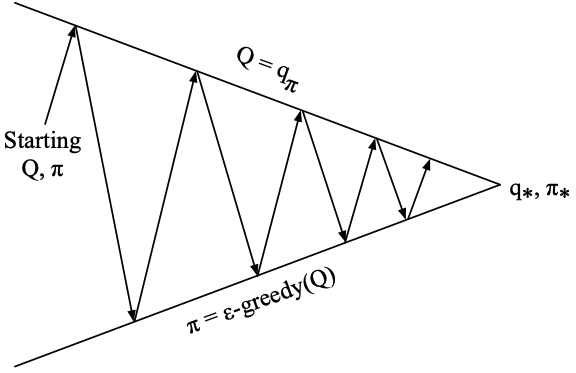
\includegraphics[scale=0.4]{images/eval_improve.png}
	\caption{ Description of the iterative policy improvement and policy evaluation using an $\varepsilon$-greedy policy.\citep{silver2015rl} Which can be proven to converge to the optimal policy in an MDP and q-value function in an MDP.}
	\label{fig:eval_improvement}
\end{figure}

\subsection{Model-Based vs Model-Free}

In general, reinforcement learning algorithms can be considered as model-free or model-based (though this line may sometimes be blurry). In model-based reinforcement learning the agent is learning a representation of the environmental dynamics, while in model-free reinforcement learning the agent is only tasked with learning the reward landscape in state-action space.

\

A model in this case would be a representation of how the environmental states will react to action taken by the agent. In this, an agent would be able to query its own model of the environment with a chain of possible actions to then be able to plan multiple time-steps into the future. Though, the model-free techniques have the future rewards encoded into their value estimates, model-based reinforcement learning has found much success within the field. \citep{moerland2022model} In this report we will be exclusively focussing on model-free algorithms.

\subsection{Example: Tabular q-learning}

To illustrate a solution to a MDP with reinforcement learning, we will consider the Frozen Lake environment from OpenAI \textit{Gymnasium} \citep{kwiatkowski2024gymnasium}. In this environment, an agent must navigate from a starting position to a goal position on a frozen grid, avoiding holes that would end the episode. The environment consists of a \(4 \times 4\) grid-world with the following specifications:

\begin{itemize}
    \item \(\mathcal{S} = \{1, 2, \dots, 16\}\): The set of 16 possible states, each representing a unique cell on the grid.
    \item \(\mathcal{A} = \{\text{RIGHT}, \text{DOWN}, \text{LEFT}, \text{UP}\}\): The set of 4 possible actions.
    \item Rewards, \(\mathcal{R}\):
    $$
    \mathcal{R} = \begin{cases}
        1, & \text{if the agent reaches the goal} \\
        0, & \text{otherwise}
    \end{cases}
    $$
\end{itemize}

\begin{figure}
	\centering
	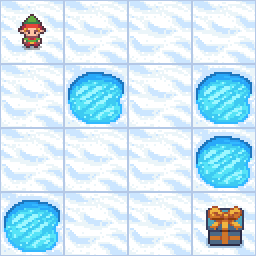
\includegraphics[scale=0.5]{images/frozen_lake_frame.png}
	\caption{Screenshot from FrozenLake \citep{kwiatkowski2024gymnasium}}
	\label{fig:frozen_lake}
\end{figure}

We will be using a tabular q-learning with a $\varepsilon$-greedy policy in order to solve this environment. What tabular q-learning requires is the storage of state-action values estimates, in other words, we require a table of q-values. From the specifications of the environment, this will be a matrix of dimension $16 \times 4$. As depicted in Figure \ref{fig:eval_improvement} we require some starting point for our q-values, which we choose to be $0$.

\

Through experience, we seek to learn what actions we should take in particular states of the environment. Therefore, we define the following update equation based on the Bellman equation for the value of the state-action pair:

\begin{equation}\label{eq:q_update}
    q(s_t, a_t) \leftarrow r_t + \gamma  \max_{a' \in \mathcal{A}(s_{t+1})} q(s_{t+1}, a')
\end{equation}

To demonstrate the learning of done by the agent we can plot a heat map of each state in the environment based on the q-value of the most rewarding action. Intuitively, we should see a heat map the depicts states near the reward with a higher maximum  state-value action. This is depicted in Figure \ref{fig:frozen_lake_q_learning}.

\begin{figure}[htp]
    \centering
    \begin{subfigure}{0.3\textwidth}
        \centering
        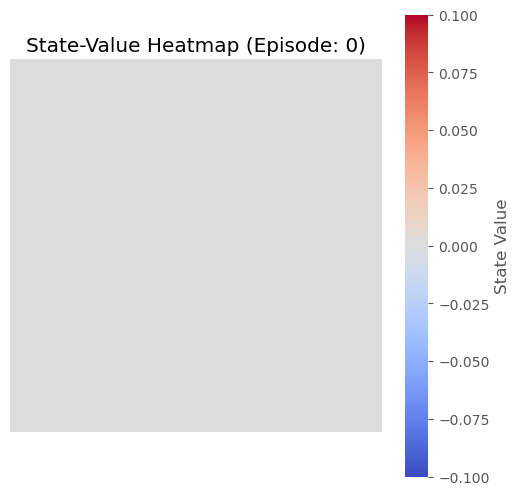
\includegraphics[width=\linewidth]{images/frozen_0.png}
        \caption{}
        \label{fig:t0}
    \end{subfigure}
    \hfill
    \begin{subfigure}{0.3\textwidth}
        \centering
        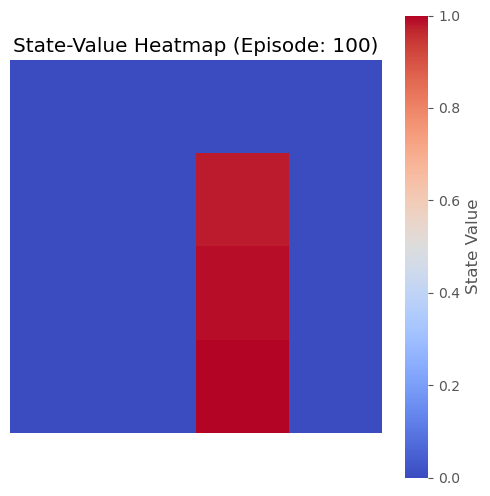
\includegraphics[width=\linewidth]{images/frozen_100.png}
        \caption{}	
        \label{fig:t100}
    \end{subfigure}
    \hfill
    \begin{subfigure}{0.3\textwidth}
        \centering
        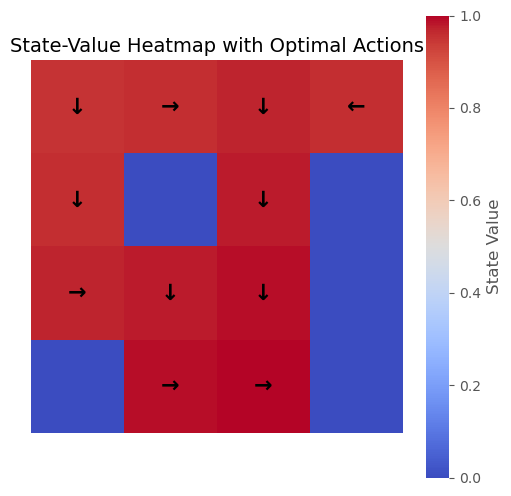
\includegraphics[width=\linewidth]{images/frozen_with_actions.png}
        \caption{}
        \label{fig:t200}
    \end{subfigure}
    
    \caption{Maximum action value state map of the frozen lake environment using tabular q-learning with exponentially decaying $\varepsilon$-greedy policy before episode 0 (\ref{fig:t0}), 100 (\ref{fig:t100}) and 200 (\ref{fig:t200}). The final plot (\ref{fig:t200}) has the optimal action indicated on the state with an arrow in the direction of that action. }
    \label{fig:frozen_lake_q_learning}
\end{figure}

\

In Figure \ref{fig:frozen_lake_q_learning}, we observe that through the random exploration of the environment the agent is able to find a corridor of high value actions seen in Figure \ref{fig:t100}. After an additional 100 episodes, the value of the actions in this corridor have been propagated throughout the environment, apart from the states that contain the obstacles. The difficulty of this environment is the sparsity of the rewards. The agent is only rewarded when getting to the goal, meaning that the only way the agent can make good decisions early in the episode is by bootstrapping the values that have been learned through random exploration.

\

Further, we can see that the greedy action in each state depicted in Figure (\ref{fig:t200}) describe a path through the environment that is optimal to get to the desired reward location, therefore we can say that this tabular q-learning algorithm has indeed solved this MDP with no prior knowledge about the environment or policy needed.

\subsection{Deep RL Algorithms}\label{sec:deep_rl}

The problem with the approach of tabular learning is that the table used to store our estimates of the q-values becomes intractable as the state and action space grow. A solution that has been used to solve this problem is using so-called ``deep'' methods. This means that we use neural networks as function approximators. What exactly these networks approximates vary depending on the algorithm, but can be the policy, q-values or values of the states. The salient point of using neural networks is that we no longer store large tables of aggregated historical data - we use the the agent experience to refine and tweak the set of parameters of our neural network which means the storage space of the machinery we use to solve these reinforcement learning problems does not grow significantly with increases to the state or action space.

\subsubsection{Deep Q-Learning}

The foundational work in the field of deep reinforcement learning was done by \citet{mnih2013playing}, in which they proposed the \textbf{Deep q-network (DQN)}. While previous approaches attempted to use non-linear function approximations for reinforcement learning \citep{tsitsiklis1996temporal}, this work represents the first instance of a neural network solving a complex problem in the domain of reinforcement learning.

\

The challenge with using neural networks for Q-learning lies in the fact that the agent must learn both the dynamics of the environment and the policy that maximises reward simultaneously. This results in a moving target problem. In standard supervised learning, the theoretic objective surface remains constant during optimisation; however, in reinforcement learning, objective evolves as the agent updates its estimates of the environment change. This makes it difficult to converge on an optimal solution, especially with non-linear function approximators.

\

Further, neural networks generally do not train very well high correlated data. In RL, the temporal experience of the agent is high correlated - where I am not has a large effect on where I can be next. 

\

To address these issues, \citet{mnih2013playing} introduced two key mechanisms in the DQN:

\begin{enumerate}
	\item \textbf{Target Network}: Instead of using the q-network directly to update itself, DQN maintains a separate target network that is a periodically frozen copy of the q-network. The q-network is used to select actions, while the target network generates Q-value estimates, which provide a more stable objective surface.
	\item \textbf{Experience Replay}: Rather than using consecutive experiences from the environment for training (which introduces correlations between data points), DQN stores past experiences in a replay buffer. During training, experiences are sampled randomly from this buffer, breaking the temporal correlation in the data. This process also improves sample efficiency, as each experience is reused multiple times, maximising learning from each interaction with the environment.

\end{enumerate}

The loss function used to update the q-network in DQN is based on the temporal difference (TD) error, given by:

\begin{equation}
L(\theta) = \mathbb{E}_{(s, a, r, s') \sim B} \left[ \left( y - Q(s, a; \theta) \right)^2 \right],
\end{equation}

where $y = r + \gamma \max_{a'} Q(s', a'; \theta_\text{target})$ is the target value computed using the target network parameters $\theta_\text{target}$, and $B$ is the replay buffer. The goal is to minimize this TD error by updating the q-network parameters $\theta$, encouraging the network to improve its estimates of the Q-values over time.

\

These innovations allowed DQN to achieve breakthrough performance on challenging tasks, such as playing Atari games from pixel input, which had previously been out of reach for reinforcement learning algorithms. \citep{mnih2013playing}

\subsubsection{Deep Recurrent Q-Learning}\label{sec:drqn}

While DQN demonstrated remarkable results, it assumes that the environment is fully observable, meaning the agent has access to all relevant information about the current state. However, in many real-world environments, the agent operates under partial observability, where only part of the information about the current state is available at any given time. For example, an agent navigating through a maze may not know its exact location without a full view of the environment.

\

To address this limitation, \textbf{Deep Recurrent Q-Learning (DRQN)} was introduced \citep{hausknecht2015deep}. DRQN combines the structure of DQN with recurrent neural networks (RNNs), allowing the agent to maintain an internal memory of previous observations, which can be used to infer hidden aspects of the state. By incorporating a recurrent layer, such as a Long Short-Term Memory (LSTM) \citep{hochreiter1997long} or Gated Recurrent Unit (GRU) \citep{chung2014empirical}, DRQN can process sequences of observations over time, making it better suited to environments with partial observability.

\

The Q-value estimate in DRQN is modified as follows:

\begin{equation}
Q(s_t, a_t; \theta, h_{t-1}) = f(s_t, h_{t-1}; \theta),
\end{equation}

where $h_{t-1}$ is the hidden state from the previous time step, and $f$ is the RNN function parameterised by $\theta$. The hidden state $h_{t-1}$ is updated at each time step, allowing DRQN to form a context over time and make informed decisions in partially observable environments.

\

The DRQN training process is similar to DQN, including the use of experience replay and a target network to stabilise training. However, the replay buffer in DRQN is adapted to store entire sequences (trajectories) rather than individual transitions, enabling the RNN to learn temporal dependencies. The training loss is computed by sampling sequences from the replay buffer and back-propagating the error through time \citep{werbos1990backpropagation}, allowing the agent to learn from temporally-extended experience.

\

DRQN extends the capabilities of DQN to a wider range of environments by equipping the agent with a memory mechanism. This allows it to excel in tasks where full observability is not guaranteed, making it more applicable to complex, real-world scenarios.

\subsubsection{Actor-Critic} 

Methods of Q-learning form part of \textbf{value-based learning}, where the task of the agent is to estimate the reward landscape of the state-action pairs for a given environment. In contrast, \textbf{policy-based methods} seek to learn the optimal policy directly within a MDP by parameterising the policy itself rather than relying on value estimates of state-action pairs.

\

The fundamental algorithm in this category is \textbf{REINFORCE} \citep{williams1992simple}. This is a Monte-Carlo-based method, where at the end of each trajectory, the cumulative returns $G_t = \sum_{k=0}^{T} \gamma^k R_{t+k+1}$ for a given action in each state encountered are fully observed.

\

The REINFORCE algorithm adjusts the parameters of the policy $\pi_\theta(a|s)$ by increasing the probability of actions that led to high returns and decreasing it for those leading to low returns. Mathematically, this adjustment is achieved by updating the policy parameters $\theta$ in the direction of the gradient of the expected return:

\begin{equation}
\theta \leftarrow \theta + \alpha \nabla_\theta J(\theta),
\end{equation}

where $\alpha$ is the learning rate, and $J(\theta) = \mathbb{E}_{\pi_\theta} [G_t]$ represents the expected return under the policy $\pi_\theta$. Using the \textbf{policy gradient theorem} \citep{sutton1999policy}, this gradient can be expressed as:

\begin{equation}
\nabla_\theta J(\theta) = \mathbb{E}_{\pi_\theta} \left[ G_t \nabla_\theta \log \pi_\theta(a_t | s_t) \right].
\end{equation}

In practice, this expectation is estimated from a single trajectory by applying the following update rule:

\begin{equation}
\theta \leftarrow \theta + \alpha G_t \nabla_\theta \log \pi_\theta(a_t | s_t).
\end{equation}

This adjustment rule intuitively increases $\pi_\theta(a_t | s_t)$ when the return $G_t$ is high (reinforcing the likelihood of actions that yield high rewards) and decreases it when $G_t$ is low. The reliance on a Monte Carlo approach makes REINFORCE unbiased but often results in high variance in the updates, which can make convergence slower. Techniques such as using \textbf{baselines} can be introduced to reduce this variance, where a baseline $b(s_t)$ is subtracted from $G_t$ to adjust the update as follows:

\begin{equation}
\theta \leftarrow \theta + \alpha (G_t - b(s_t)) \nabla_\theta \log \pi_\theta(a_t | s_t).
\end{equation}

This baseline, often set to an estimate of the state value $V(s_t)$, helps centre the updates, making the learning process more stable by only reinforcing actions that perform above the baseline. This is known as the critic.

\

Actor-critic methods maintain two neural networks. The actor maps the observations into the probability distribution over actions and can be understood as the policy network. The critic is an estimate of the rewards of the state action pairs state-action. The critic is then trained on the rewards obtained from the environment, similarly to how a DQN is trained. And the actor is trained based on the temporal-difference update generated by the critic network. 

\subsubsection{Proximal Policy Optimisation (PPO)}

While actor-critic methods offer an effective way to combine the benefits of both value-based and policy-based learning, they can suffer from instability. In particular, if the policy updates are too large, the agent's behaviour can oscillate, leading to divergence rather than convergence. This instability arises because a large update can significantly change the policy, moving it too far from the policy that generated the value estimates, thereby making the value function inaccurate for the updated policy.

\

To address this issue, a regularisation approach known as \textbf{Trust Region Policy Optimisation (TRPO)} was introduced \citep{schulman2015trust}. TRPO limits the update step size to constrain how far the new policy deviates from the old policy, which reduces the risk of instability. This is achieved by optimising a surrogate objective function while enforcing a constraint on the Kullback-Leibler (KL) divergence between the old and new policies. The TRPO objective can be expressed as:

\begin{equation}
\max_\theta \mathbb{E}_{s \sim \pi_\text{old}} \left[ \frac{\pi_\theta(a|s)}{\pi_\text{old}(a|s)} A^{\pi_\text{old}}(s, a) \right],
\end{equation}

subject to the constraint:

\begin{equation}
\mathbb{E}_{s \sim \pi_\text{old}} \left[ D_\text{KL}(\pi_\text{old} \| \pi_\theta) \right] \leq \delta,
\end{equation}

where $A^{\pi_\text{old}}(s, a)$ is the advantage function calculated using the old policy $\pi_\text{old}$, and $\delta$ is a threshold that restricts the KL divergence to maintain a trust region around the old policy. This constraint limits drastic changes in the policy, ensuring smoother updates and more stable learning.

\

While effective, TRPO can be complex to implement due to its reliance on a second-order optimisation technique to enforce the KL constraint. To simplify this, \textbf{Proximal Policy Optimisation (PPO)} \citep{schulman2017proximal} was developed. PPO uses a modified objective function that replaces the strict KL constraint with a clipped surrogate objective, making the algorithm both simpler to implement and computationally efficient while retaining the stability benefits of TRPO.

PPO’s objective function is given by:

\begin{equation}
L^{\text{CLIP}}(\theta) = \mathbb{E}_{s \sim \pi_\text{old}, a \sim \pi_\theta} \left[ \min \left( r(\theta) A^{\pi_\text{old}}(s, a), \text{clip}(r(\theta), 1 - \epsilon, 1 + \epsilon) A^{\pi_\text{old}}(s, a) \right) \right],
\end{equation}

where the probability ratio $r(\theta)$ is defined as:

\begin{equation}
r(\theta) = \frac{\pi_\theta(a|s)}{\pi_\text{old}(a|s)}.
\end{equation}

The clipping function limits the change in $r(\theta)$ within the interval $[1 - \epsilon, 1 + \epsilon]$, where $\epsilon$ is a hyper-parameter usually set to $0.3$. By applying this clipping, PPO discourages excessively large updates, thus providing a balance between exploration and policy stability. The objective function ensures that if the update moves the policy ratio outside of this range, the advantage term is effectively set to zero, preventing excessive updates.

\

In practice, PPO achieves a robust performance by iteratively sampling trajectories, estimating the advantage values using the critic, and optimising the clipped objective to update the actor network. The simplicity and effectiveness of PPO has made it a popular choice for many RL tasks.

\newpage

\section{Multi-Agent Reinforcement Learning (MARL)}

While single-agent reinforcement learning has achieved significant success, many real-world problems involve multiple interacting agents, which are collectively referred to as \textit{multi-agent systems}. These systems require agents to collaborate or compete to achieve complex objectives. For instance, in smart power grids, agents coordinate to manage electricity distribution by synchronising generators, storage, utilities, and consumers, enabling the integration of renewable energy sources \citep{yu2024safe}. In disaster rescue scenarios, autonomous robots work together to map disaster areas, locate survivors, and deliver essential supplies. \citep{song2023disaster} In this section, we will extend the tools developed for RL to tackle the unique challenges of multi-agent systems, exploring methods for effective coordination, competition, and resource sharing among agents.

\subsection{Multi-agent system}

A multi-agent system consists of an \textit{environment} and \textit{agents} that interact in the environment to achieve some goal. This is similar to agent agent-environment loop that was described in the first section only that now the combination of all $n$ agents within the environment will affect the underlying state. This loop is described in Figure \ref{fig:agents_environment_loop}. 

\begin{figure}
	\centering
	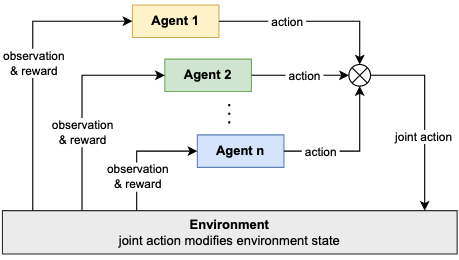
\includegraphics[scale=0.6]{images/multiple_agent_environment.png}
	\caption{Agents-environment loop \citep{albrecht2024marl} in multi-agent systems}
	\label{fig:agents_environment_loop}
\end{figure}

\

The collection of states, actions, observations, and rewards are formally defined within \textit{game models}. Different types of game models exist, and we introduce common game models used in MARL in Section \ref{sec:game_models}, including  stochastic games, and partially observable stochastic games. A solution for a game model consists of a set of policies for the agents that satisfies certain desired properties. The exact properties that are desired are formally solution concepts, forms of solution concepts are described in Section \ref{sec:solution_concepts}.

\subsection{Game models}\label{sec:game_models}

In a very similar fashion to how our description of the reinforcement learning task then fed into our description of a Markov decisions process - we will too be placing a multi-agents systems into sequential decision process frameworks that are called game models. 

\

A multi-agent system can be formalised in many different ways \citep{oliehoek2016concise} depending on whether the environment is fully observable, how agents' goals are correlated, or whether communication and coordination between agents are allowed. The partially observable stochastic game (POSG) \citep{hansen2004dynamic} is defined by a tuple $\left\langle\mathcal{I}, \mathcal{S}, \rho^0,\left\{\mathcal{A}_i\right\}, P,\left\{\mathcal{O}_i\right\}, O,\left\{R_i\right\}\right\rangle$, where $\mathcal{I}$ is a (finite) set of agents indexed as $\{1, \ldots, n\}, \mathcal{S}$ is a set of environment states, $\rho^0$ is the initial distribution over state space $\mathcal{S}, \mathcal{A}_i$ is a set of actions available to agent $i$, and $\mathcal{O}_i$ is a set of observations of agent $i$. 

\

We denote a joint action space as $\mathcal{A}=\times_{i \in \mathcal{I}} \mathcal{A}_i$ and a joint observation space of agents as $\mathcal{O}=\times_{i \in \mathcal{I}} \mathcal{O}_i$. Therefore, $P: \mathcal{S} \times \mathcal{A} \rightarrow \Delta(\mathcal{S})$ denotes the transition probability from a state $s \in \mathcal{S}$ to a new state $s^{\prime} \in \mathcal{S}$ given agents' joint action $\mathbf{a}=\left\langle a_1, \ldots, a_n\right\rangle$, where $\mathbf{a} \in \mathcal{A}$. With the environment transitioning to the new state $s^{\prime}$, the probability of observing a joint observation $\mathbf{o}=\left\langle o_1, \ldots, o_n\right\rangle$ (where $\mathbf{o} \in \mathcal{O}$ ) given the joint action $\mathbf{a}$ is determined according to the observation probability function $O: \mathcal{S} \times \mathcal{A} \rightarrow \Delta(\mathcal{O})$. Each agent then receives an immediate reward according to their own reward functions $R_i: \mathcal{S} \times \mathcal{A} \times \mathcal{S} \rightarrow \mathbb{R}$. Similar to the joint action and observation, we could denote $\mathbf{r}=\left\langle r_1, \ldots, r_n\right\rangle$ as a joint reward. If agents' reward functions happen to be the same, i.e., they have identical goals, then $r_1=r_2=\ldots=r_n$ holds for every time step. In this setting, the POSG is reduced to a decentralised partially observable MDP (Dec-POMDP) \citep{oliehoek2016concise}. 

\

If at every time step the state is uniquely determined from the current set of observations of agents, i.e., $s \equiv \mathbf{o}$, the Dec-POMDP is reduced to a Dec-MDP. If each agent knows what the true environment state is, the Dec-MDP is reduced to a Multi-agent MDP. If there is only one single agent in the set of agents, i.e., $\mathcal{I}=\{1\}$, then the Multi-agent MDP is reduced to an MDP and the Dec-POMDP is reduced to a POMDP. Due to the partial observability, MARL methods often use the observation-action history $\tau_{i, t}=\left\{o_{i, 0}, a_{i, 0}, o_{i, 1}, \ldots, o_{i, t}\right\}$ up to time step $t$ for each agent to approximate the environment state.

\subsection{Solution concepts}\label{sec:solution_concepts}

Solution concepts in MARL define optimal policies for agents interacting in a game. Solutions are often joint policies that optimise returns for each agent based on conditions related to expected rewards and mutual interactions. Many of these solutions use the notion of best responses, where a best-response policy maximises an agent's expected returns given the policies of other agents. \citep{albrecht2024marl}Equilibrium concepts, such as minimax (for zero-sum games), Nash equilibrium, and correlated equilibrium, ensure that no agent can improve its return by unilaterally deviating from the current strategy. Games can have unique or multiple equilibria, resulting in varying expected returns, so achieving an equilibrium does not necessarily maximise returns for all agents. 

\

Additional refinement criteria, such as Pareto optimality, social welfare, and fairness, are often applied to equilibria to select more desirable solutions, such as a Nash equilibrium that is also Pareto-optimal. \citep{albrecht2024marl} Another solution concept, no-regret learning, considers the alternative returns agents could have obtained by using different actions in past interactions; in the limit, a no-regret policy ensures that the average regret approaches zero. Finally, computing a Nash equilibrium in general-sum games is a PPAD-complete problem, indicating that efficient MARL algorithms for finding Nash equilibria may not exist for general games.


\subsection{Environment Types}

In MARL, the types of environments agents interact in are generally classified as cooperative, competitive, or mixed. In a cooperative environment, agents share a common objective, and their rewards are aligned to encourage collaboration toward mutual goals. This setup promotes coordinated strategies where agents work together to maximise a joint reward. Conversely, in a competitive environment, agents have opposing goals, and interactions are often modelled as zero-sum games, where one agent’s gain is another agent’s loss. Here, agents act in direct competition, optimising their strategies to maximise individual rewards, sometimes at the expense of others. 

\

Mixed environments combine elements of both cooperation and competition, where agents may collaborate in certain aspects or with certain agents while competing in others. These environments lead to partially aligned and partially conflicting objectives, requiring agents to balance cooperative strategies with competitive tactics, depending on the situation and the rewards at stake.


\subsection{Training and Execution Modes}

MARL algorithms are generally categorised based on the information available to agents during training and execution of policies. In some cases, MARL training may be limited to using only local information available to each agent independently, known as \textit{decentralised training}. Alternatively, the training process may access global information from all agents within the environment, a setup known as \textit{centralised training}. After the training phase, another question arises: What information will agents use during execution? Specifically, agents may condition their policies only on their local observations, referred to as \textit{decentralised execution}, or they may have access to global information from all agents, called \textit{centralised execution}. Below, we outline the main categories of MARL algorithms based on these training and execution modes.

\paragraph{Centralised Training and Execution} In centralised training and execution, both the learning and execution of agent policies rely on centrally shared information among agents. This may include the local observation histories of all agents, shared models of the environment, joint value functions, or even the policies themselves. Centralised training and execution require agents to have access to more information than typically allowed in a POSG since agents receive global rather than local information. Central learning, for instance, can reduce a multi-agent game to a single-agent problem by using joint observation data to train a unified policy over the combined action space, effectively controlling all agents. This approach benefits from having access to a larger observation space, which can be useful for handling partial observability and coordinating complex actions. However, centralised learning has limitations:

\begin{enumerate}
	\item a joint reward for all agents may be challenging to define
	\item the joint action space grows exponentially with the number of agents, making the learning process computationally demanding
	\item agents may be distributed physically or virtually, making communication with a central policy impractical
\end{enumerate}

For instance, in autonomous vehicle control, real-time data exchange from all surrounding vehicles may not be feasible, and even if achieved, the complexity of centralised control would make the policy learning unmanageable. Here, decentralised control, where each vehicle operates as an independent agent, is generally more practical.

\paragraph{Decentralised Training and Execution} In decentralised training and execution, both the training and deployment of agent policies are fully independent, relying only on local information observed by each agent. This approach is often used in settings where centralised information sharing is impractical or unavailable. A prime example of decentralised learning occurs in financial markets, where individual traders lack full visibility into others' actions or their effects on the market, observing only partial impacts. \citep{albrecht2024marl} One method, known as \textit{independent learning}, has each agent treating the rest of the environment - including other agents - as a dynamic, non-stationary component and applying single-agent reinforcement learning techniques. Independent learning scales well by avoiding the joint action space's exponential growth, and it is particularly well-suited to distributed agents that cannot communicate, such as in remote environments. However, this approach presents three main challenges:

\begin{enumerate}
	\item agents cannot leverage information about other agents’ behaviours during training or execution
	\item training suffers from non-stationarity introduced by concurrent learning among agents
	\item agents cannot differentiate between environmental stochasticity and the impact of other agents’ actions
\end{enumerate}

\paragraph{Centralised Training and Decentralised Execution} The third category, centralised training and decentralised execution (CTDE), is widely used in MARL. Here, agent policies are trained with shared, global information but are designed for independent deployment, requiring only local observations for action selection. During training, CTDE algorithms leverage shared observations across agents to improve policy accuracy, yet once deployed, agents act independently based solely on local data. This approach is prevalent in deep MARL as it allows policies to benefit from more informative value functions in a computationally efficient way. A common CTDE method is the multi-agent actor-critic algorithm, where a centralised critic uses joint observations to estimate values with high accuracy, enhancing learning. At execution, the critic is no longer required, and each agent’s policy relies only on its own observations, allowing fully decentralised deployment.


\subsection{Challenges of MARL}

Multi-agent reinforcement learning faces unique challenges due to factors such as conflicting objectives, differing partial observations of the environment, and the concurrent adaptation of their policies. Below, we outline some of the main challenges associated with MARL:

\begin{itemize}
    \item \textbf{Non-stationarity due to Learning Agents} One of the defining characteristics of MARL is non-stationarity, arising from the continuously evolving policies of agents as they learn. This non-stationarity introduces a moving target problem, as each agent’s policy is dynamically adjusting in response to other agents’ policies, which are also concurrently adapting. This can create complex, cyclic interactions and even unstable learning dynamics, making it difficult for agents to achieve stable convergence. Furthermore, agents may learn at different rates due to variations in their rewards or local observations, which can exacerbate the instability. Managing non-stationarity robustly is a key requirement for MARL algorithms and remains an active area of research.
    \item \textbf{Optimality of Policies and Equilibrium Selection} Determining optimal policies in MARL is challenging due to the interdependence of agents' policies on one another. In single-agent reinforcement learning, a policy is considered optimal if it maximises expected returns from each state. In contrast, MARL requires solution concepts such as equilibrium solutions, where each agent’s policy is optimal with respect to the others. Unlike in single-agent cases where all optimal policies yield the same expected return, in a multi-agent system, agents may receive different rewards, resulting in multiple possible equilibrium points, each with different outcomes for each agent. Thus, agents must effectively ``negotiate'' during learning to select which equilibrium to converge to. Developing algorithms that reliably guide agents towards desired equilibrium solutions is a core objective in MARL research.
    \item \textbf{Multi-Agent Credit Assignment} Credit assignment in reinforcement learning refers to identifying which past actions were responsible for a particular reward. In MARL, this problem becomes even more complex as it involves not only temporal credit assignment but also the challenge of determining which agent’s actions contributed to the received reward. Efficiently resolving multi-agent credit assignment is crucial for learning accurate policies in shared reward scenarios.
    \item \textbf{Scalability with Number of Agents} The action space in a multi-agent system grows exponentially with the number of agents, especially if each agent has unique action options. For instance, in cooperative tasks like level-based foraging \citep{papoudakis2021benchmarking}, adding an agent introduces an additional action variable to control a robot, exponentially increasing the number of potential joint actions. Early MARL research often limited experiments to two agents to avoid scalability issues, and even with modern deep learning techniques, MARL implementations typically involve between 2 and 10 agents. \citep{albrecht2024marl} Developing scalable algorithms capable of handling larger numbers of agents in a computationally feasible and robust way remains an essential objective in MARL research.
\end{itemize}

\subsection{MARL Algorithms}\label{sec:marl_algorithms}

In this section, we will examine some popular MARL algorithms. These build on the single agent algorithms that were introduced and explained in Section \ref{sec:deep_rl}. 

\subsubsection{Independent Q-learning}

A basic approach one can take to extend a single-agent RL algorithm to a multi-agent algorithm is to simply ignore the influence that other agents have on the environment. This approach is called Independent Q-learning (IQL) \citep{tan1997MultiAgentRL}. In this algorithm, all agents will act completely independently.

\

\begin{equation}
L(\theta^i) = \mathbb{E}_{(s^i, a^i, r^i, s'^i) \sim B} \left[ \left( y^i - Q(s^i, a^i; \theta^i) \right)^2 \right],
\end{equation}

where $y^i = r^i + \gamma \max_{a'} Q(s'^i, a'^i; \theta^i_\text{target})$, where we are required to now condition the components of the model on the agent $i$.

\

The original implementation of this algorithm was done in \citet{tan1997MultiAgentRL} where the independent learning was compared to agent's learning with communication of instantaneous information episodic experience and learned knowledge. However, as we discuss in the next section, this communication is not learnt but specified a-priori. The cooperation that was introduce using communication enabled the agent's to converge to a policy that solved the predator-prey problem. Even from this early stages the fundamental issues of MARL were present when the enlarged sensory information was shown to interfere with learning. The communication created a larger observational space for each agent, due to this they were unable to learn a policy in this larger space. \citep{tampuu2015multiagent}

\

Modern extensions to this algorithms can be found in \citet{tampuu2015multiagent} where IQL was combined with DQN's to create independent deep q-learning. In this, the agent's were tasked at playing the game of Pong, where the emergence of commutative or cooperative behaviour was observed based on the reward structure. Where strategies that enabled longer rallies - returning balls to the centre of the opponent's side - emerged if the agent's were rewarded for longer rallies. While competitive strategies emerged when agent's were rewarded for their opponent's missing the ball.

\

The primary benefit of IQL is its simplicity, as it treats multi-agent problems in a decentralised manner. Each agent learns and executes its policy independently, which avoids complex coordination mechanisms and makes it scalable to larger agent populations. However, this decentralised approach faces challenges in non-stationary environments, where each agent's actions influence others, creating shifting dynamics that can lead to instability and difficulty in convergence, particularly in competitive or highly interactive settings.

\subsubsection{Independent Proximal Policy Optimisation}

Still in the realm of independent learning, \textbf{Independent Proximal Policy Optimisation (IPPO)} \citet{witt2020independent} adapts the principles of Independent Q-Learning to policy-based methods, specifically leveraging PPO for each agent. In IPPO, each agent independently applies PPO to update its own policy without explicit coordination or shared representations across agents. A core adjustment required to transition PPO to IPPO is the independent treatment of each agent’s policy and value updates.

\

In contrast to Independent Q-Learning, IPPO employs parameter sharing as a means to enhance scalability and learning efficiency, particularly in environments with homogeneous agents. Parameter sharing is applied by using a single neural network as a centralised critic, which is augmented with an agent-specific identifier at the input layer to distinguish between agents. This approach, initially explored by \citet{gupta2017cooperative}, extends single-agent reinforcement learning algorithms for multi-agent applications. Parameter sharing here is done by using a shared critic for all agents, which receives each agent’s observation and identifier as input, enabling the critic to generalise across agents’ perspectives while maintaining unique policies per agent. For heterogeneous environments, agent-specific identifiers play an essential role in conditioning the shared network’s responses to different agents. IPPO applies parameter sharing across both the agent’s critic and actor networks, which helps to reduce computational costs while still allowing for distinct policies for each agent. 

\

IPPO has demonstrated impressive performance, outperforming other state-of-the-art MARL algorithms across various difficulty levels in StarCraft multi-agent challenge environments \citep{witt2020independent}. A key factor contributing to this performance is PPO’s policy clipping mechanism, which is thought to mitigate some of the instability caused by environmental non-stationarity that tends to hinder independent learning algorithms. Clipping the policy loss helps limit the extent to which each agent’s policy changes during each update, stabilising learning in the face of changing policies of other agents.

\

IPPO utilises centralised learning only in the form of parameter sharing in the actor and critic networks, while maintaining decentralised execution, as the trained policies can operate independently at runtime. This CTDE balance enables IPPO to handle multi-agent tasks while retaining the benefits of independent learning.

\subsubsection{Multi-Agent Proximal Policy Optimization (MAPPO)}

\textbf{Multi-Agent Proximal Policy Optimization (MAPPO)}\citep{chao2021surprising} offers an alternative framework to extend PPO to the multi-agent setting. MAPPO incorporates a centralised critic network that receives the global state as input, representing the combined observations of all agents, while each agent has its own actor network for decentralised policy execution. In environments with homogeneous agents, these actor networks often use parameter sharing to further streamline training. 

\

The shift from PPO to MAPPO requires a few specific mathematical modifications to the PPO objective to enable centralised training and decentralised execution. MAPPO introduces a centralised value function, \( V_{\theta}(s) \), where \(s\) is the global state, allowing the critic to learn the overall value of the shared environment. The actors, in turn, use the centralised critic’s evaluation as a baseline to stabilise policy updates, applying PPO’s clipped surrogate objective:

\begin{equation}
L(\theta) = \mathbb{E}_t \left[ \min \left( r_t(\theta) \hat{A}_t, \text{clip}(r_t(\theta), 1 - \epsilon, 1 + \epsilon) \hat{A}_t \right) \right],
\end{equation}
where \( r_t(\theta) = \frac{\pi_{\theta}(a_t | s_t)}{\pi_{\theta_\text{old}}(a_t | s_t)} \) is the probability ratio and \( \hat{A}_t \) is the advantage function computed from the centralised critic. The centralised critic’s value estimates help mitigate non-stationarity by providing each agent with a consistent measure of overall state value, even as other agents’ policies evolve.

\

MAPPO achieves high performance in both final returns and sample efficiency, rivalling other methods on a range of cooperative multi-agent tasks. This success suggests that properly configured PPO algorithms can serve as a competitive baseline for cooperative MARL tasks. \citep{chao2021surprising}.

\

MAPPO also falls under the CTDE paradigm. Here, the centralised critic is utilised only during training to evaluate joint states, and each agent’s policy is then executed independently at execution time, without needing access to global information. The primary distinction between IPPO and MAPPO lies in the critic’s structure: while IPPO relies on independently trained critics (with optional parameter sharing), MAPPO uses a centralised critic network that serves all agents.

\newpage

\section{MARL with Communication}

The RL agent-environment loop is not merely a framework for solving sequential decision problems, but the pattern observed matches with modern theories of the dopamine system in the brain \citep{paul2011understanding} as well as classical conditioning from the field of Phycology \citep{gowda2024bridging}. Further, the very structure of the node in a neural network is based on the way in which neurons in the brain are believed to perform computations. The salient point is that advancements in the field have been inspired by the human experience. Therefore, considering how humans over come problems of credit assignment, scaling and non-stationarity is a justified starting point to solve these problems in MARL. The fundamental mechanism humans use to do this is \textbf{communication}.

\ 

The communication considered in these multi-agent systems are protocols that are \textbf{learnable and dynamic}, as opposed to \textbf{static and predefined}. To this end, the solving the domain-specific action policies becomes a joint learning challenge, where agents employ reinforcement learning to maximise environmental rewards and simultaneously utilise machine learning techniques to develop efficient and effective communication. \citep{zhu2024survey}

\

\citet{zhu2024survey} identify three key components for distinguishing models within the Comm-MADRL field: problem setting, communication process, and training process. The problem setting encompasses elements that are specific to communication, such as constraints on communication bandwidth or channel reliability, as well as aspects not directly related to communication, such as the structure of the reward system, which shapes each agent's goals and behaviours. The communication process includes the mechanisms by which agents determine both when to communicate and what information to convey, which may vary depending on the environment and objectives. Finally, the training process addresses the strategies used to learn both the agents' individual behaviours and their communication protocols, which is essential for optimising coordinated action within MARL.

\

Based on these components we will discuss nine research questions that arise in Comm-MADRL. These questions and dimensions are outlined in Table \ref{table:comm_marl_dimensions}. These dimensions are identified and discussed extensively in \citet{zhu2024survey} which fully covers the state of communication in MARL. The approach taken in this paper differs from \citet{zhu2024survey} in the sense that we do not seek to cover the field at large, but rather use a small number of representative models to aid the discussion on these dimensions. These models include fundamental algorithms such as RIAL and DIAL \citep{foerster2016learning}, CommNet \citep{sukhbaatar2016commnet}. As well as adaptions and more contemporary models such as IC3Net \citep{singh2018ic3net}, BiCNet \citep{peng2017bicnet}, NeurComm \citep{chu2020NeurComm} and HAMMER \citep{gupta2022HAMMER}. 

\

The particular neural network and training structure is not explicitly the focus of this section, though many of these features naturally arise in the dimensions of a Comm-MARL model. If the reader seeks a description of thees models entirely they can consult Appendix \ref{sec:models}, but this section is not needed to understand the following discussion on the dimensions of Comm-MARL algorithms.

\begin{table}[hbt]
    \centering
    \begin{tabular}{|>{\centering\arraybackslash}m{3cm}|>{\centering\arraybackslash}m{1cm}|>{\arraybackslash}m{6cm}|>{\centering\arraybackslash}m{3cm}|}
        \hline
        \textbf{Component} & \textbf{Index} & \textbf{Question} & \textbf{Dimension} \\
        \hline
        Problem Setting
        & 1 & What kind of behaviours are desired to emerge with communication? & Controlled Goals \\
        \cline{2-4}
        & 2 & How to fulfil realistic requirements? & Communication Constraints \\
        \cline{2-4}
        & 3 & Which type of agents to communicate with? & Communicatee Types \\
        \hline
        Communication Processes
        & 4 & When and how to build communication links among agents? & Communication policy \\
        \cline{2-4}
        & 5 & How to combine received messages? & Message combination \\
        \cline{2-4}
        & 6 & Which piece of information to share? & Communicated messages \\
        \cline{2-4}
        & 7 & How to integrate combined messages into learning models? & Inner integration \\
        \hline
        Training Processes 
        & 8 & How to train and improve communication? & Learning methods \\
        \cline{2-4}
        & 9 & How to utilise collected experience from agents? & Training schemes \\
        \hline
    \end{tabular}
    \caption{Proposed dimensions and associated research questions in Comm-MADRL}
    \label{table:comm_marl_dimensions}
\end{table}

\subsection{Controlled Goals}

Agents within a reinforcement learning environment are tasked at achieving their desired goals and interests. The goal of communication within these systems is to enable larger reward returns. Therefore, the reward configuration of the environment and the communication within the environment are tightly coupled. Communication models have been tested in cooperative, competitive and mixed environments.

\paragraph{Cooperative and global} \citet{foerster2016learning} developed two cooperative environments in order to evaluate the RIAL and DIAL models - Switch Riddle and MNIST Game. The switch riddle environment is based on a riddle from \citet{wu2002prisoners}. The problem is:

\begin{quote}
One hundred prisoners have been newly ushered into prison. The warden tells them that starting tomorrow, each of them will be placed in an isolated cell, unable to communicate amongst each other. Each day, the warden will choose one of the prisoners uniformly at random with replacement, and place him in a central interrogation room containing only a light bulb with a toggle switch. The prisoner will be able to observe the current state of the light bulb. If he wishes, he can toggle the light bulb. He also has the option of announcing that he believes all prisoners have visited the interrogation room at some point in time. If this announcement is true, then all prisoners are set free, but if it is false, all prisoners are executed. The warden leaves and the prisoners huddle together to discuss their fate. Can they agree on a protocol that will guarantee their freedom?
\end{quote}

Even when simplified from one hundred prisoners to three the solution to this riddle is not clear. The communication that is encouraged is the convergence to a stable protocol that solves the environment. And indeed RIAL and DIAL converge to a solution for three prisoners. Moreover, the communication in these models are discretised which means one can evaluate exactly the protocol that has emerged to solve the switch riddle problem. This is shown in Figure \ref{fig:switch_riddle_solution}.

\

\begin{figure}
	\centering
	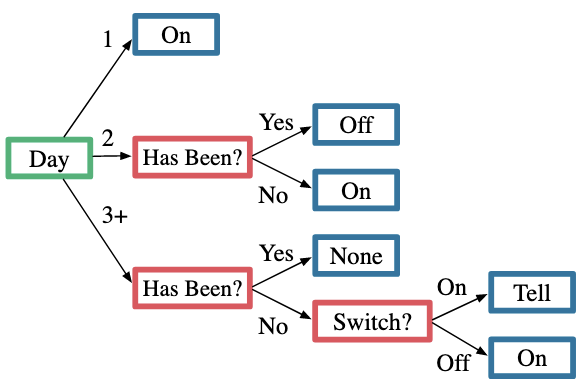
\includegraphics[scale=0.8]{images/switch_riddle}
	\caption{Image from \citet{foerster2016learning} demonstrating the learned protocol from RIAL and DIAL when each model had solved the Switch Riddle environment. The decision tree can be interpreted from a three option choice of the day outlined in green. Binary choices are outlined in red and the final action is outlined in blue. }
	\label{fig:switch_riddle_solution}
\end{figure}

Still within the cooperative setting, \citet{sukhbaatar2016commnet} assessed their model within the Traffic Junction environment which was too used in \citet{singh2018ic3net}. In this, cars enter into a grid where the they are assigned three possible routes - left, right or straight. The cars are also equipped with two actions - gas or break. If two cars collide (ie. occupy the same space in the grid) each car gets $-10$ reward and the simulation will carry. The key is that the cars have a small visibility range, but can communicate to all cars.

\

The ideal behaviour that this environment seeks to encourage is a protocol that can broadcasts information that reduces the effect of the partial observability. Indeed, \citet{sukhbaatar2016commnet} found that the communication channel in CommNet was particularly active when agent's were in particular states - like the states near the junction of the roads, but the agents preferred not to communicate. Which gives the impression that a noisy, busy communication channel was disruptive to the tasks and a smaller amount of clear information is more useful when solving this task. IC3Net \citep{singh2018ic3net} too used this environment and found similar results with respect to the usage of the communication channel but faster convergence to a protocol in simulations using their model.

\paragraph{Cooperative with local rewards}

\citet{peng2017bicnet} tested BiCNet in StartCraft Combat games with local rewards. The idea with cooperation with local rewards is that global rewards structures can ignore the need for locally coordinating agents. This type of distinction is needed in a more complicated environment like StarCraft. It was found that agents were able to learn high level coordination strategies  like cover attack. The essence of cover attack is to let one agent draw fire or attentions from the enemies, meanwhile, other agents take  advantage of this time period or distance gap to output more  harms. The difficulty of conducting cover attack lies in how  to arrange the sequential moves of multiple agents in a coordinated hit and run way which it was found that IC3Net was able to do.

\paragraph{Competitive and mixed with local rewards}

IC3Net \citep{singh2018ic3net} has the advantaged of individualised rewards, unlike RIAL, DIAL \citep{foerster2016learning} and CommNet \citep{sukhbaatar2016commnet}. This means that the model can also be tested in competitive and mixed environments. \citet{singh2018ic3net} tested the model in the predator-prey environment. The environment has a fixed prey and $n$ predators. The competitiveness of the environment is adjusted based on the reward structure. In cooperative scenarios, the more predators on a prey the greater the reward, and the opposite in the competitive variation. In the competitive setup, one sees the communication gates (See Appendix \ref{sec:models} for details) used to reduce the communication omitted by the agents. Meaning that the model learns \textbf{not} to communicate with opposing agents. In this competition is was found that communicating agents out performed non-commutative teams.

\subsection{Communication Constraints}

Within Comm-MARL there can be constraints placed on the communication within the model or environment. These constraints are often imposed to create an analogy within real world communication. For example, typically we consider language to be communication with a finite lexicon - discrete message constraints are placed on communication channels to create an analog to this. Communication channels can be noisy in real life - we can talk in a crowd with (literal) noise in the background - and so message signals sent can also have some random fluctuation added to it.

\paragraph{Constrained communication} DIAL and RIAL \citep{foerster2016learning} have a communication channel capacity introduced in the model. In the case of the Switch Riddle, this communication channel is constrained to a single bit. This is a bandwidth constraint. In DIAL, we also have messages that have noise added to them - which is an example of a corrupted channel. The interesting feature of this channel is that the communication is through the noisy channel but the feedback is not. Similarly, in HAMMER \citep{gupta2022HAMMER} the communication protocol was trained through a noisy channel aiming to create more purposeful messages.

\

These noise constrains are implemented in the discretise-regularise unit (DRU) \citep{foerster2016learning} (See Appendix \ref{subsec:dial_rial} for more details). The usage of this unit was actually for training purposes rather than for simulation of human interaction. The DRU is used in models that require end-to-end differentiability but who seek to enforce a discrete communicative protocol. During learning, in order to pass parameter gradients between neural networks the DRU adds noise to messages (and passing them through a sigmoid function) in order for message values that are close to 0 to be corrupted more than messages with large absolute values. The usage for these types of `confident' protocols is that they are easily discretised during execution where all messages are passed through an indicator function: $DRU(m) = \mathbbm{1}_{[0, \infty)}$. 

\

A sort of meta-constraint will always be present in these models as an assumption of the form of the messages, whether that be a dimension of real numbers, so a certain way in which the messages are output. Thus, we are only considering the discretising of messages and a noisy channel to be the constraints we consider since these are most common in the literature and are closely related to human language.

\paragraph{Unconstrained communication}
CommNet \citep{sukhbaatar2016commnet} introduces no constraint on the message that is sent. The messages are aggregations of the internals states of each agent in the environment (apart from themselves) but there is no constraint on the value of the message that is to be sent or with whom the agents can send the message to. However, these a hyper constraint given by the choice of dimension of the message. For example, in CommNet the messages are the same dimension as the hidden state. To our knowledge there has been no model that aims to learn this hyper-parameter. \citet{singh2018ic3net} is similar in this unconstraint communication channel but this model has the key feature of a learnt gating mechanism of outgoing messages. This allows agents to learn not to communicate but does not have any explicit loss attached to it and is therefore not considered to be a constraint. 

\subsection{Communicatee Types}

Communicatee type determines the criteria of the agent that one can send a message to. There are naturally, location constraints with communication in real life but there can be other conventions that dictate the communication within a muti-agent system. In a software development team, it is not always necessary for the developers to communicate directly with each other and could rather have a system in place where another employee is responsible for aggregating the communication from the team and passing on only what is relevant to each team member, like a project manager. In this case, the communication is mediated through a proxy.

\paragraph{Learning other agents to communicate with} IC3Net \citep{singh2018ic3net} have no constraint on the agents that can be communicated with. This is since all agents will be receiving an average of the hidden state of the other agents, which is the same as CommNet \citep{sukhbaatar2016commnet}. The difference is the gating introduced by \citet{singh2018ic3net} which allows agents to learn a function that can remove all communication with specific agents.

\paragraph{Nearby agents} In NeurComm \citep{chu2020NeurComm} the MAS is represented as a graph. Where agents are considered nodes who can only communicate with their neighbours in the graph. The agent then receives their own local observation as well as the concatenation of all neighbour's messages as the ``state'' input to its neural network. For agent $i$ with a neighbourhood $N_i$ it would use:

\begin{equation}
	s_i^t = o_i^t \cup m_{N_i}^t 
\end{equation}

Where $m_{N_i}^t = \{ m_j^t : j \in N_i \}$, as the input to its policy or actor network.

\paragraph{Proxy} A proxy is a virtual agent that plays a role in facilitating communication but does not directly affect the environment. Using a proxy as the communicatee means that agents will not directly communicate with each other, instead messaged are constructed from a proxy based on information from the environment. In the HAMMER model \citep{gupta2022HAMMER} there is a centralised agents that receives all observation as input to its neural network. In other words, the central agent receives $\mathbf{o^t} = [o^t_1, \hdots, o_J^t]$ with $J$ agents in the environment at time $t$. The central agent is then responsible for generating personalised messages for each agent in the form of single real number or a real-valued vector with a small number of dimensions. This proxy agent can then be trained using the gradients computed by the individual agents, or using the global rewards of the agents. This represents a differentiable vs reinforced learning scheme which will be discussed in Section \ref{sec:learning_methods}. 

\begin{figure}
	\centering
	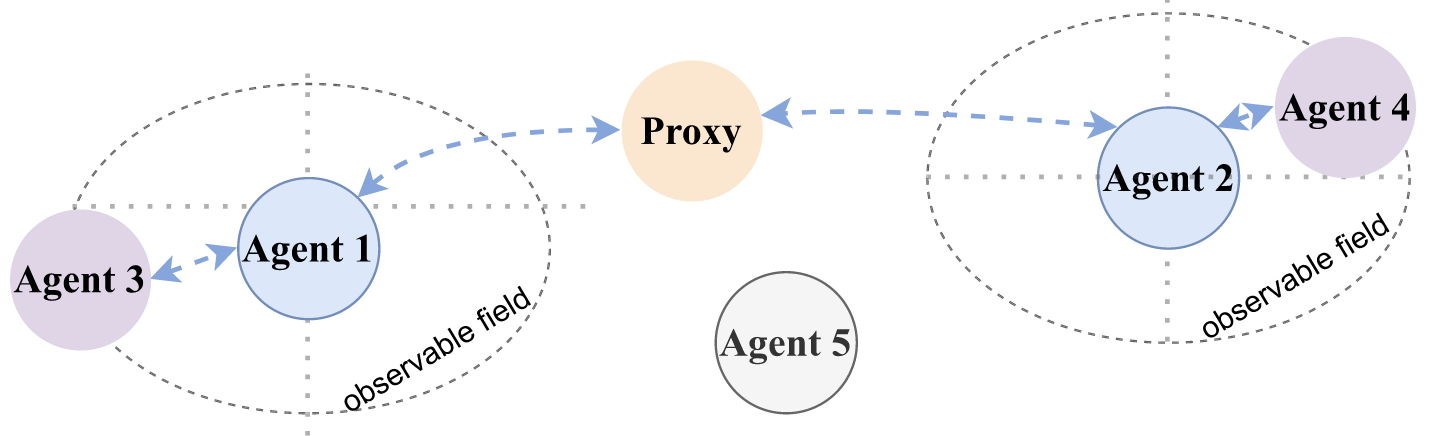
\includegraphics[scale=0.5]{images/communicatee.png}
	\caption{Image from \citet{zhu2024survey} demonstrating the difference between communication among nearby agents within the observable field, and communication between agents between a mediating proxy agent. These represent two different kinds of communicatee types in Comm-MARL}
	\label{fig:communicatee}
\end{figure}

\subsection{Communication policy}

A communication policy defines a set of communicative actions, which can be modelled in different ways. For example, a communication action can be represented as a vector of binary values, where each value indicates whether communication between agents is available. These policies can be learned of predefined:

\paragraph{Predefined full communication} In DIAL and RIAL \citet{foerster2016learning} the agents have full access to communicate with all agents. When viewed as a graph - this means that each agent is connected to every other agent so any message that gets sent by one agent is broadcast to the entire network. BiCNet \citep{peng2017bicnet} obtains a full communication graph but through other agents. Since, the communication within this model is using recurrent connections between the hidden states of agents. Similar to recurrent connections through time, only the preceding agent is able to send a message, but the effect of the previous recurrent connection is still present in the hidden state that is being communicated. Thus, there is an implicit full communication structure in this model. 

\paragraph{Predefined local policies} In NeurComm \citep{chu2020NeurComm}, communication is only available to agents' within a neighbourhood. The implementation then employs a spatial dimension to determine which agents are in a neighbourhood, this would of course change if agent's can move in an environment. Thus, this is a predefined policy, but implemented locally.

\paragraph{Learnt individual control} IC3Net \citep{singh2018ic3net} has a gating mechanism that enables the agents to learn to communicate or not to communicate with a other agents. In this sense, their communication policy is learnt during training. A crucial point is that the learning is done individually. Each agent is tasked with performing this same task.

\begin{figure}
	\centering
	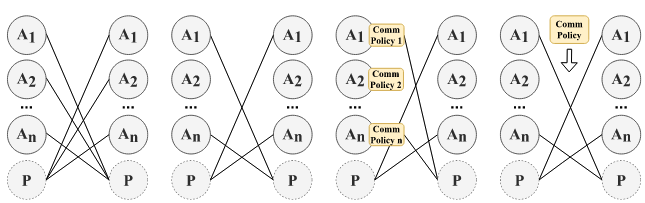
\includegraphics[scale=0.5]{images/communication_policies.png}
	\caption{Architectural description of communication policies examined \citet{zhu2024survey}. }
	\label{fig:communication_policies}
\end{figure}

\subsection{Communicated messages}

After establishing communication links among agents through a communication policy, agents should determine which specific information to communicate. This information can derive from historical experiences, intended actions, or future plans, enriching the messages with valuable insights. Consequently, the communicated information can expand the agents’ understanding of the environment and enhance the coordination of their behaviours. In the dimension of communicated messages, an important consideration is whether the communication includes future information, such as intentions and plans. This kind of information, being inherently private, often requires an (estimated) model of the environment to effectively simulate and generate conjectured intentions and plans.

\paragraph{Existing knowledge} In this category agents share knowledge about their environment. This can be in the form of low dimensional encoding of their hidden states. This is particularly prevalent in models based on RNN's \citep{sukhbaatar2016commnet, peng2017bicnet, singh2018ic3net}. The architecture allows for the encoding of previous information, as well as present observation to then be combined into a message for other agents. RIAL and DIAL \citep{foerster2016learning} have message as output in their RNN's as opposed to communicating hidden states. Intuitively, this means that messages are more explicitly learnt.

\paragraph{Imagined future knowledge} In NeurComm \citep{chu2020NeurComm} agents do not only communicate their existing knowledge but some prediction about their future actions. Existing knowledge is communication in a similar manner to other models where the is some aggregation of the hidden states. However, future knowledge that the agent passes on is in the form of a policy fingerprint. A policy finger is some statistical representation of the policy, like the sufficient statistics. The agent encodes information about future actions in particular states that can be used by other agents to plan their policies. The problem in this scheme can be the moving target, if one agent communicated a policy finger print, that informs another agent's policy which it too communicates. This issue did not arise in NeurComm. \citep{chu2020NeurComm}


\subsection{Message combination}

When agents receive more than one message, current works often aggregate all received messages to reduce the input for the action policy. Message Combination determines how to integrate multiple messages before they are processed by an agent’s internal model. If a proxy is involved, each agent receives already coordinated and combined messages from the proxy, eliminating the need for further message combination. If no proxy is presented, each agent independently determines how to combine multiple messages. Since communicated messages encode the senders’ understanding of the learning process or the environment, some messages can be more valuable than others. 

\paragraph{Equally valued} In this category, messages received by agents are treated without preference, meaning they are assigned equal weights or simply no weights at all. Without having preferences, agents can concatenate all messages, ensuring no loss of information, though it may significantly expand the input space for the action policy. Equally values messages are found in RIAL and DIAL \citep{foerster2016learning}, CommNet \citep{sukhbaatar2016commnet} and IC3Net \citep{singh2018ic3net}. 

\paragraph{Unequally valued} In BiCNet \citep{peng2017bicnet} the message received from agents that have closer indexes will have a greater influence on the message that is being communicated. The messages in this model flow through recurrent connection in the RNN. Thus, the message sent from an agent indexed further away will have less impact on the agent's actions. Social convention-like roles emerged from these unequal weightings. For instance, certain agents might be more critical in relaying positioning information, while others may prioritise attack strategies, resulting in a form of "social convention" where some agents’ messages carry more significance in coordinating team behaviour.

\subsection{Inner Integration}

Inner Integration refers to how information received from other agents is incorporated into an agent’s learning model, which may include a policy function, a value function, or both. In most existing literature, these messages are treated as additional observations, augmenting each agent's decision-making inputs.

\

\paragraph{Policy-Level Integration}
Policy-level integration enables agents to modify their action selection based directly on the messages received from other agents. In this setup, the messages act as supplementary inputs to the policy function, effectively allowing agents to align their actions with the anticipated behaviours of their peers. This coordination mechanism means that agents no longer act independently but rather exploit shared information to improve collective performance. Policies are commonly learned using policy gradient methods, such as REINFORCE, where episodic rewards are collected and used to train the policy at the end of each episode.\citet{sukhbaatar2016commnet} and \citet{singh2018ic3net} exemplify this approach by training policy networks that incorporate inter-agent messages, which guide actions in multi-agent cooperative tasks.

\

\paragraph{Value-Level Integration}
Value-level integration involves incorporating messages directly into the value function, which in turn informs the agent’s action choices by evaluating the expected long-term reward of different actions. In this category, agents use a value function to assimilate messages, typically implemented as part of a Q-learning or DQN-like framework. Here, messages become inputs that condition the value function, which estimates the Q-values for each action based on both the agent’s observations and the received messages. The action with the highest Q-value is then selected, thus leveraging the messages to influence decision-making indirectly through the value estimates. Notable examples of this approach include RIAL and DIAL \citep{foerster2016learning}, which use differentiable inter-agent learning structures to enhance coordination. In these frameworks, messages allow agents to share critical state information or learned signals that improve the accuracy of the Q-value predictions, thereby optimising the action choices in cooperative settings.

\

\paragraph{Policy and Value-Level Integration}
Integrating messages within both the policy and value functions simultaneously enables agents to utilise communication comprehensively across both decision-making and evaluation processes. This dual integration is often implemented using actor-critic methods, where messages can directly influence both the policy and the value networks. By treating received messages as additional inputs for both models, agents can jointly optimise their actions based on the current observations and message-prompted internal states. An example is BiCNet \citep{peng2017bicnet}, where received messages are incorporated at both the policy and value levels, enhancing agents’ abilities to dynamically adjust their strategies based on interactions with others. In some cases, messages are combined with local observations to produce a new set of internal states that are shared with both the actor and critic networks, thereby establishing a more cohesive and responsive learning model that adapts to both immediate and strategic needs.

\

Additionally, HAMMER \citep{gupta2022HAMMER} use an actor-critic model (PPO) to learn the communication. The proxy in this model has communication its actions so it can therefore use the reward or gradient feedback to then train its communicative mechanism.

\subsection{Learning methods}\label{sec:learning_methods}

Learning methods determine which type of machine learning techniques are used to learn a communication protocol. The learning of communication is at the centre of Comm-MARL and can benefit from the advancements in the machine learning. If some assumptions about communication are made, such as being able to calculate the derivatives with respect to the message generator function and the communication policy, then the training of communication can be integrated into the overall learning process of agents. This integration allows for the use of fully differentiable methods for backpropagation. Other machine learning techniques, including reinforcement learning can too be used to learn the a communication protocol. 

\paragraph{Differentiable} Neural networks are end to end differentiable which means that networks can pass gradients in order to improve the feedback mechanisms present in their communication. In DIAL \citep{foerster2016learning} the gradient of the message sent by the receiver is propagated back to the sender. This is akin to a nod when talking to someone. In this set-up, the communicatees are agents while in HAMMER \citep{gupta2022HAMMER}, the communication is mediated through the a central agent. This agent can too receive the gradient feedback from each agent given the personalised message it sent. What is crucial is that all messages and computations are fully-differentiable so we are able to pass around gradients.

\paragraph{Reinforced} Models can also use methods of reinforcement learning in order to learn communication protocols. In this case, the gradients are based on the reward feedback from the environment. In this, the messages can be seen as included in the action space for each agent. The issue in this is that the reward feedback is now a black-box - in the same way that the action to reward relationship is in regular reinforcement learning. RIAL \citep{foerster2016learning} still learned a solution policy to the three agent Switch Riddle but was not able to achieve any learning when the size of the environment increased to four agents. A similar less effective training was seen in HAMMER \citep{gupta2022HAMMER} when using reinforced learning techniques.

\subsection{Training schemes}

This dimension focuses on how to utilise the collected experiences (such as observations, actions, rewards, and messages) of agents to train their action policies and communication architectures in a Comm-MARL system. Agents can train their models in a fully decentralised manner using only their local experience. Alternatively, when global information is accessible, the experiences of all agents can be collected to centrally train a single model that controls all agents. However, each approach has inherent challenges. Fully decentralised learning must cope with a non-stationary environment due to the changing and adapting behaviours of agents, while fully centralised learning faces the complexities of joint observation and policy spaces. As mentioned before, CTDE methods create a compromise between these two extreme methods.

\paragraph{Centralised learning and decentralised execution} In CTDE approaches, the experiences of all agents are collectively used for optimisation. Gradients derived from the joint experiences guide the learning of local policies. However, once training is complete, only the policies are needed and gradients can be discarded, facilitating decentralised execution. When agents are assumed to be homogeneous, meaning they have identical sensory inputs, actuators, and model structures, they can share parameters. Parameters sharing reduces the overall number of parameters, potentially enhancing learning efficiency compared to training in separate processes. Despite sharing parameters, agents can still exhibit distinct behaviours because they are likely to receive different observations at the same time step. This is the most common traning methods in Comm-MARL and is observed in \citet{foerster2016learning, sukhbaatar2016commnet, singh2018ic3net}. 


\paragraph{Decentralised Learning} In decentralised learning the agent only has access to local observations and chooses actions based on these observations. Within Comm-MARL, the agents have access to messages are communicated to them. In this sense, there may be information in those messages that is not in the immediate proximity of that agent. In NeurComm \citep{chu2020NeurComm} this training regiment is used. Where global information can be present through cascaded neighbourhood communications.

\newpage

\section{Experiment}

What is clear from the current state of Comm-MARL is methods that using a differentiable learning methods out perform those using a reinforced learning technique. Intuitively, this is because gradient feedback from a message is a more direct indicator of the usefulness of the message than reward feedback from the environment. Messages can be interpreted differently from agent to agent so learning to communicate in a reinforced fashion would seem to be less efficient. However, in many practical applications parameter sharing is in feasible \citep{wong2022deep}. Typically, parameter sharing is done by each agent using the same neural network for training while local observational input induces different behaviour. This means that agents cannot learn different policies. \citep{terry2023revisiting} This issue is often circumvented by adding an `agent input' to the neural networks, meaning that the network will input some identifier of the agent. This approach is limited, however, in that without modification it does not allow parameter sharing to be applied to environments where the action space and/or observation space are heterogeneous.

\

If we do not assume parameter sharing among agents can effective communication still arise? This is the question that \citet{pina2024fully} seek to answer. In this section we will examine the model used in \citet{pina2024fully} as well as  confirm the results, and discuss the implications thereof. The goal of this section is to discuss whether effective communication can be achieved without the use of parameter sharing.

\subsection{Method}

From the description of the goal of the experiment we can identify two different dimensions for investigation within the model: communication and parameter sharing. The presence and absence of those components creating four treatments: No parameter and no communication (NPS), no parameter sharing and communication (NPS+COMM), parameter sharing and no communication (NPS) and parameter sharing and communication (PS+COMM). These models are tested in two environments: Predator Prey and Traffic Junction. \citep{sukhbaatar2016commnet}

\

In the Predator-Prey (Figure \ref{fig:predator_prey}) environment, agents are \emph{predators} which aim to capture prey by coordinating their movements. The predators are rewarded for successfully capturing prey, which is achieved when a predator comes within a specified capture radius of a prey agent. Predators are encouraged to cooperate with each other to maximise the chances of capturing prey. There are variants of this environment where prey are also artificial agents, however, in the investigation the prey are fixed in position and the predators seek them out. Thus, this is a purely cooperative environment.

\

The Traffic Junction environment (Figure \ref{fig:traffic_junction})simulates an intersection where multiple agents (vehicles) navigate to cross safely without collisions. Each vehicle agent follows a decision-making policy to avoid crashes and minimise wait time at the junction. The environment models real-world traffic scenarios to study cooperative strategies in multi-agent systems.

\begin{itemize}
    \item \textbf{Objective:} Each vehicle aims to cross the junction as quickly as possible without causing collisions. Agents must coordinate their movements to avoid conflict at the intersection.
    \item \textbf{Actions:} Agent can choose from accelerate or break to either move along their allocated path or to stay in place for a time step. 
    \item \textbf{Rewards:} Agents receive positive rewards for successfully crossing the junction without collisions and incur penalties for delays or causing accidents.
\end{itemize}

The Traffic Junction environment provides insights into cooperative behaviour under shared constraints, such as road usage, where agents must learn to avoid collisions and efficiently cross the junction.

\begin{figure}[h]
    \centering
    \begin{subfigure}[b]{0.4\textwidth}
        \centering
        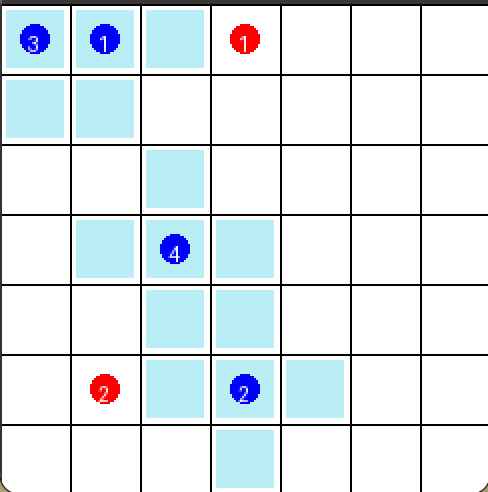
\includegraphics[width=\textwidth]{images/predetorprey}
        \caption{Predator-Prey Environment}
        \label{fig:predator_prey}
    \end{subfigure}
    \hfill
    \begin{subfigure}[b]{0.4\textwidth}
        \centering
        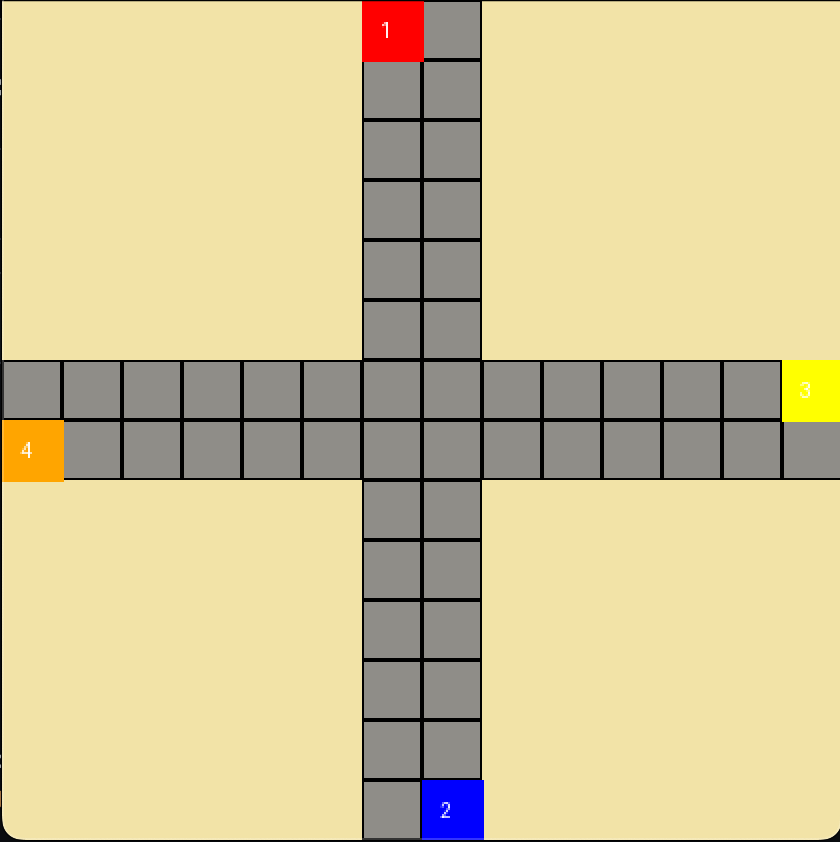
\includegraphics[width=\textwidth]{images/traffic_junction}
        \caption{Traffic Junction Environment}
        \label{fig:traffic_junction}
    \end{subfigure}
    \caption{Illustrations of the Predator-Prey and Traffic Junction environments from \citep{magym2019github}.}
    \label{fig:environments}
\end{figure}

\subsection{Model}

The model used in this investigation is based on the IQL model from Section \ref{sec:marl_algorithms}. Let us state again the loss function required for IQL:

\begin{equation}\label{eq:iql_2}
	\mathcal{L}(\theta) = \mathbb{E}_{b \sim B}\left[ (r + \gamma \max_{a'} Q(a', \theta^- - Q(ra; \theta) )^2 \right]
\end{equation}


Let us consider the environment with $N$ agents with $\mathcal{M}$ and $\mathcal{Q}$ be the set of all messages and q-values respectively. Let $f_i \to \mathcal{Q}$ and $g_i \to \mathcal{M}$. We will describe the models of each of the treatment cases individually.

\paragraph{PS+COMM} We have that 
\begin{equation}
	\{Q_i\}_{i=1}^N =\{f_i(o_i, m_{-i}m a_i; \theta)\}_{i = 1}^N
\end{equation}
Where $m_{-i}$ corresponds to the message from all agents except $i$, these messages are produced by $g_i$ parameterised by $\mu$:

\begin{equation}
	m_{-i} = \{ g_j(o_j; \mu) \}^N_{j = 1, \ j \neq i} \wedge m_i = g_i(o_i; \mu) 
\end{equation}
As per (\ref{eq:iql_2}), we can define the loss function for the learning problem as
\begin{equation}
\begin{aligned}
\mathcal{L}_i(\theta, \mu) & =r+\gamma \max _{a_i^{\prime}} Q_i\left(o_i^{\prime}, m_{-i}^{\prime}, a_i^{\prime} ; \theta^{-}\right)-Q_i\left(o_i, m_{-i}, a_i ; \theta\right) \\
& =r+\gamma \max _{a_i^{\prime}} f_i\left(o_i^{\prime},\left\{g_j\left(o_j^{\prime} ; \mu^{-}\right)\right\}_{j=1, j \neq i}^{j=N}, a_i^{\prime} ; \theta^{-}\right) \\
& -f_i\left(o_i,\left\{g_j\left(o_j ; \mu\right)\right\}_{j=1, j \neq i}^{j=N}, a_i ; \theta\right) .
\end{aligned}
\end{equation}

From the above, we can write $\mathcal{L}_i(\theta, \mu) \equiv \mathcal{L}_i\left(f_i(\cdot ; \theta, \mu), g_i(\cdot ; \mu)\right)$, and then we can also write the backpropagation rules for the gradients as
\begin{equation}
\begin{gathered}
\nabla_\theta \mathcal{L}_i=\frac{\partial \mathcal{L}_i}{\partial f_i} \frac{\partial f_i}{\partial \theta}+\frac{\partial \mathcal{L}_i}{\partial g_i} \frac{\partial g_i}{\partial \theta}=\frac{\partial \mathcal{L}_i}{\partial f_i} \frac{\partial f_i}{\partial \theta} \\
\nabla_\mu \mathcal{L}_i=\frac{\partial \mathcal{L}_i}{\partial f_i} \frac{\partial f_i}{\partial \mu}+\frac{\partial \mathcal{L}_i}{\partial g_i} \frac{\partial g_i}{\partial \mu}
\end{gathered}
\end{equation}

and from this, it follows that the parameters of the networks are updated as:

\begin{equation}
\begin{gathered}
\theta=\theta-\alpha \nabla_\theta \mathcal{L}_i=\theta-\alpha \frac{\partial \mathcal{L}_i}{\partial f_i} \frac{\partial f_i}{\partial \theta} \\
\mu=\mu-\alpha \nabla_\mu \mathcal{L}_i=\mu-\alpha\left(\frac{\partial \mathcal{L}_i}{\partial f_i} \frac{\partial f_i}{\partial \mu}+\frac{\partial \mathcal{L}_i}{\partial g_i} \frac{\partial g_i}{\partial \mu}\right) .
\end{gathered}
\end{equation}

This is the standard procedure for IQL with parameter sharing. 

\paragraph{NPS+COMM} We now have that:
\begin{equation}
\left\{Q_i\right\}_{i=1}^N=\left\{f_i\left(o_i, m_{-i}, a_i ; \theta_i\right)\right\}_{i=1}^N,
\end{equation}

where $m_{-i}$ corresponds once again to the messages from all agents except $i$, that are produced by a neural network denoted by a function $g_j$ with parameters $\mu_j$

\begin{equation}\label{eq:iql_ps_message}
m_{-i}=\left\{g_j\left(o_j ; \mu_j\right)\right\}_{j=1, j \neq i}^N \wedge m_i=g_i\left(o_i ; \mu_i\right)
\end{equation}

Similarly to (\ref{eq:iql_2}), we can define the loss function for the learning problem as
\begin{equation}
\begin{aligned}
\mathcal{L}\left(\theta_i, \mu_{-i}\right) & =r+\max _{a_i^{\prime}} Q_i\left(o_i^{\prime}, m_{-i}^{\prime}, a_i^{\prime} ; \theta_i^{-}\right)-Q_i\left(o_i, m_{-i}, a_i ; \theta_i\right) \\
& =r+\max _{a_i^{\prime}} f_i\left(o_i^{\prime},\left\{g_j\left(o_j^{\prime} ; \mu_j^{-}\right)\right\}_{j=1, j \neq i}^{j=N}, a_i^{\prime} ; \theta_i^{-}\right) \\
& -f_i\left(o_i,\left\{g_j\left(o_j ; \mu_j\right)\right\}_{j=1, j \neq i}^{j=N}, a_i ; \theta_i\right)
\end{aligned}
\end{equation}

Because now networks are not shared, from the above we can write:

\begin{equation}
\mathcal{L}_i\left(\theta_i, \mu_{-i}\right) \equiv \mathcal{L}_i\left(f_i\left(\cdot ; \theta_i, \mu_{-i}\right), g_{-i}\left(\cdot ; \mu_{-i}\right)\right)
\end{equation}

Thus in order to update $\mu_i$ the corresponding gradient rule in this case would have to be

\begin{equation}
\nabla_{\mu_i} \mathcal{L}_j=\frac{\partial \mathcal{L}_j}{\partial f_j} \frac{\partial f_j}{\partial \mu_i}+\frac{\partial \mathcal{L}_j}{\partial g_{-j}} \frac{\partial g_{-j}}{\mu_i}
\end{equation}

This does not make sense since agent $j$ does not share parameters with agent $i$, and thus $\mu_i$ will never be updated $\forall i \in\{1, \ldots, N\}$.

\

The parameters of a communication network $\mu_i$ of agent $i$ will never be updated if fully independent learners that do not share the parameters $\theta_i$ and $\mu_i$ learn only from their observations and incoming messages from the others. As a solution to this \citet{pina2024fully} propose instead the following learning scheme for independent communication:

\begin{equation}\label{eq:q_iql_nps}
\left\{Q_i\right\}_{i=1}^N=\left\{f_i\left(o_i, m_{-i}, m_i, a_i ; \theta_i\right)\right\}_{i=1}^N
\end{equation}

where $m_{-i}$ corresponds once again to the messages from all agents except $i$, that are produced by a function $g_j$ with parameters $\mu_j$, in the same way as in (\ref{eq:iql_ps_message}). $\mathcal{L}_i$ can now be written as:

\begin{equation}
\begin{aligned}
& \mathcal{L}_i\left(\theta_i, \mu_{-i}, \mu_i\right)= \\
& \quad=r+\operatorname{\gamma ax}_{a_i^{\prime}} Q_i\left(o_i^{\prime}, m_{-i}^{\prime}, m_i^{\prime}, a_i^{\prime} ; \theta_i^{-}\right)-Q_i\left(o_i, m_{-i}, m_i, a_i ; \theta_i\right) \\
& \quad=r+\max _{a_i^{\prime}} f_i\left(o_i^{\prime},\left\{g_j\left(o_j^{\prime} ; \mu_j^{-}\right)\right\}_{j=1, j \neq i}^{j=N}, g_i\left(o_i^{\prime} ; \mu_i^{-}\right), a_i^{\prime} ; \theta_i^{-}\right) \\
& \quad-f_i\left(o_i,\left\{g_j\left(o_j ; \mu_j\right)\right\}_{j=1, j \neq i}^{j j}, g_i\left(o_i ; \mu_i\right), a_i ; \theta_i\right),
\end{aligned}
\end{equation}

and now, we have that $\mathcal{L}_i\left(\theta_i, \mu_{-i}, \mu_i\right) \quad \equiv$ $\mathcal{L}_i\left(f_i\left(\cdot ; \theta_i, \mu_{-i}, \mu_i\right), g_{-i}\left(\cdot ; \mu_{-i}\right), g_i\left(\cdot ; \mu_i\right)\right)$, and we can now write the rules as:

\begin{equation}\label{eq:q_iql_nps}
\begin{gathered}
\nabla_{\theta_i} \mathcal{L}_i=\frac{\partial \mathcal{L}_i}{\partial f_i} \frac{\partial f_i}{\partial \theta_i}+\frac{\partial \mathcal{L}_i}{\partial g_{-i}} \frac{\partial g_{-i}}{\partial \theta_i}+\frac{\partial \mathcal{L}_i}{\partial g_i} \frac{\partial g_i}{\partial \theta_i}=\frac{\partial \mathcal{L}_i}{\partial f_i} \frac{\partial f_i}{\partial \theta_i}, \\
\nabla_{\mu_i} \mathcal{L}_i=\frac{\partial \mathcal{L}_i}{\partial f_i} \frac{\partial f_i}{\partial \mu_i}+\frac{\partial \mathcal{L}_i}{\partial g_{-i}} \frac{\partial g_{-i}}{\partial \mu_i}+\frac{\partial \mathcal{L}_i}{\partial g_i} \frac{\partial g_i}{\partial \mu_i}=\frac{\partial \mathcal{L}_i}{\partial f_i} \frac{\partial f_i}{\partial \mu_i}+\frac{\partial \mathcal{L}_i}{\partial g_i} \frac{\partial g_i}{\partial \mu_i} .
\end{gathered}
\end{equation}

Intuitively, this step solves the problem stated in Remark 1. However, now when doing the final rule, it is implied that:

\begin{equation}\label{eq:other_gradient_update}
\begin{aligned}
\nabla_{\mu_{-i}} \mathcal{L}_i & =\frac{\partial \mathcal{L}_i}{\partial f_i} \frac{\partial f_i}{\partial \mu_{-i}}+\frac{\partial \mathcal{L}_i}{\partial g_{-i}} \frac{\partial g_{-i}}{\partial \mu_{-i}}+\frac{\partial \mathcal{L}_i}{\partial g_i} \frac{\partial g_i}{\partial \mu_{-i}} \\
& =\frac{\partial \mathcal{L}_i}{\partial f_i} \frac{\partial f_i}{\partial \mu_{-i}}+\frac{\partial \mathcal{L}_i}{\partial g_{-i}} \frac{\partial g_{-i}}{\partial \mu_{-i}}
\end{aligned}
\end{equation}

From (\ref{eq:other_gradient_update}), we note the existence of a second problem (that is independent of our solution to the problem in Remark 1), since $\mu_{-i}$ would be updated as:

\begin{equation}
\mu_{-i}=\mu_{-i}-\alpha\left(\frac{\partial \mathcal{L}_i}{\partial f_i} \frac{\partial f_i}{\partial \mu_{-i}}+\frac{\partial \mathcal{L}_i}{\partial g_{-i}} \frac{\partial g_{-i}}{\partial \mu_{-i}}\right),
\end{equation}

for $N$ times, causing losses of gradient when propagating through the same values several times.

\

If fully independent agents that do not share the parameters $\theta_i$ and $\mu_i$ of their networks learn from the messages of the others, then the incoming messages will be used for backpropagation $N$ times, causing problems in the computational graph. To overcome the problem, for each agent $i$, we detach $m_{-i}$ from the computational graph, ensuring that all $\theta_i \wedge \mu_i, i \in\{1, \ldots, N\}$ are updated exactly once, according to:

\begin{equation}
\begin{gathered}
\theta_i=\theta_i-\alpha \frac{\partial \mathcal{L}_i}{\partial f_i} \frac{\partial f_i}{\partial \theta_i}\\
\mu_i=\mu_i-\alpha\left(\frac{\partial \mathcal{L}_i}{\partial f_i} \frac{\partial f_i}{\partial \mu_i}+\frac{\partial \mathcal{L}_i}{\partial g_i} \frac{\partial g_i}{\partial \mu_i}\right)
\end{gathered}
\end{equation}

As per (\ref{eq:q_iql_nps}). With this learning scheme, which can be summarised by (\ref{eq:q_iql_nps}), fully independent learning with communication and without parameter sharing can be achieved. This scheme allows all the parameters to be updated, enabling learning with communication.

\begin{figure}
	\centering
	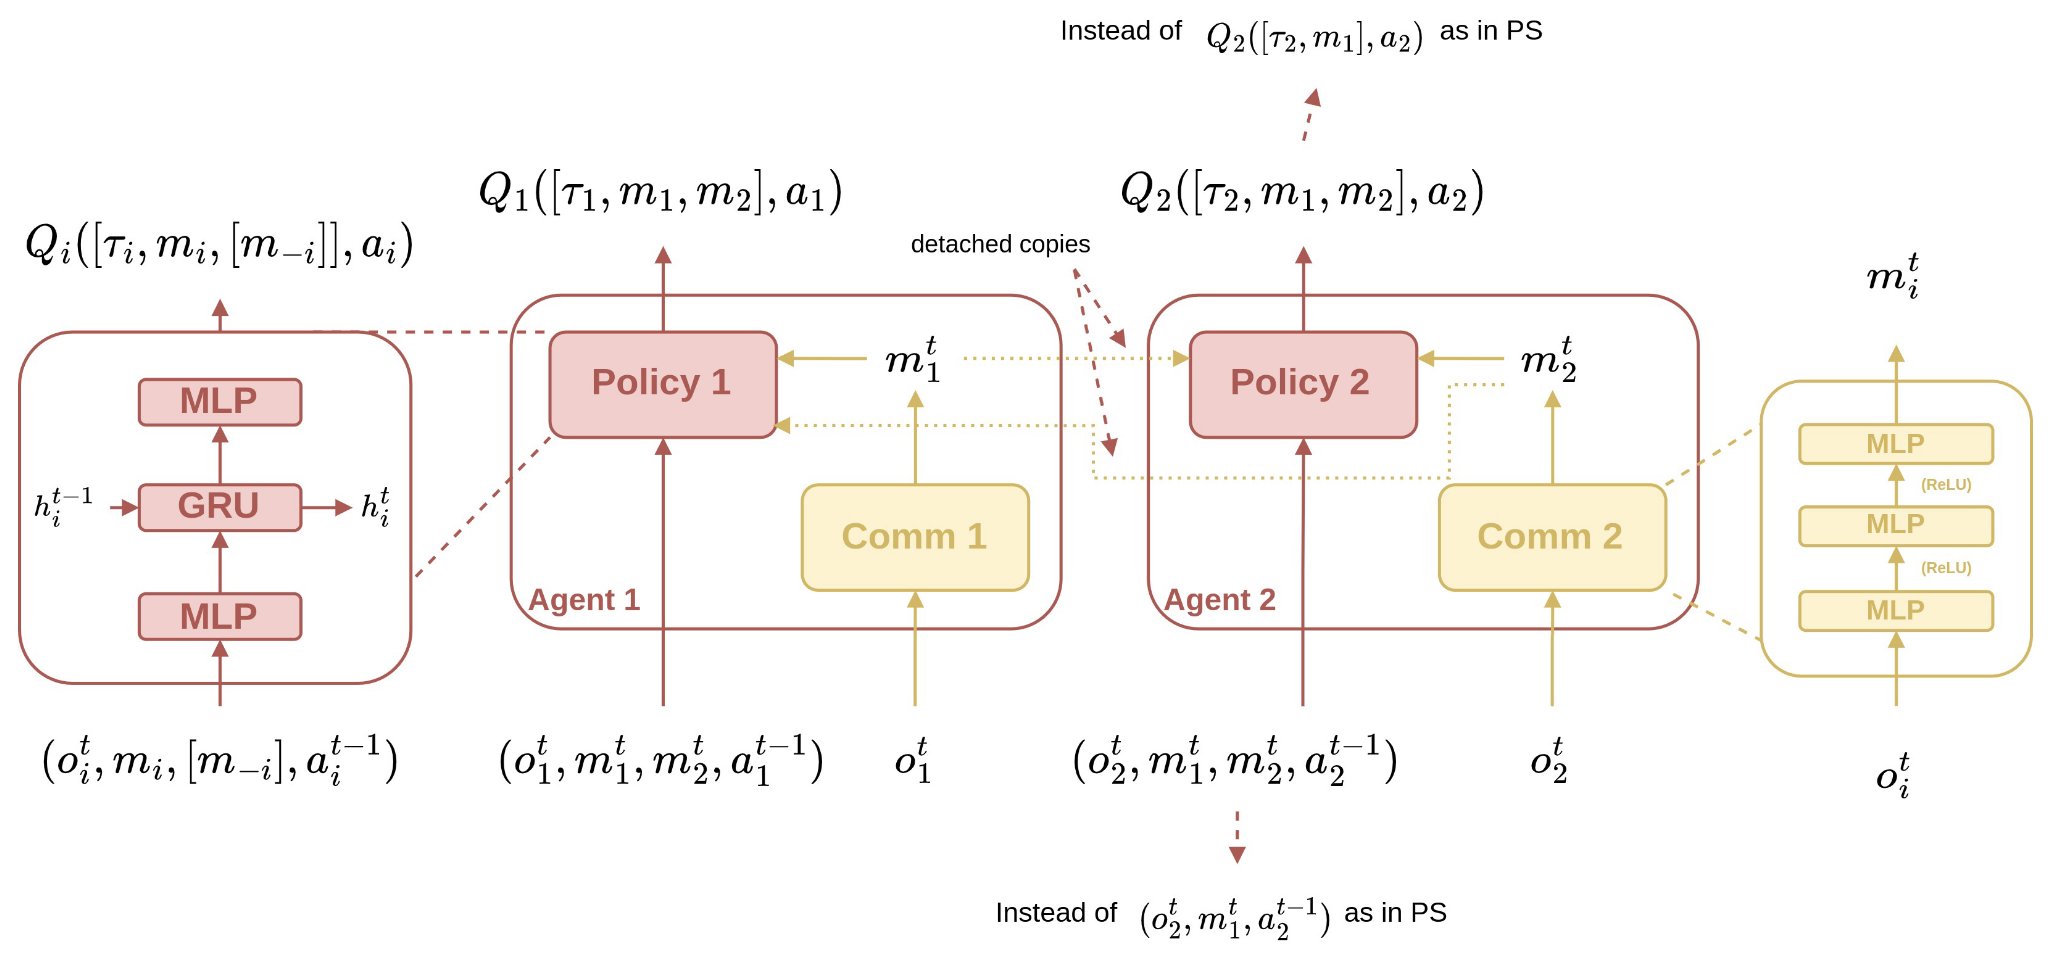
\includegraphics[scale=0.4]{images/nps_comm.png}
	\caption{Illustration of how the proposed scheme for independent communication without parameter sharing (NPS+COMM) \citep{pina2024fully} works when compared to sharing parameters (PS). The figure shows that agents that do not share parameters also need to receive their own message as input to keep the link to the computational graph of their communication network during backpropagation.}
	\label{fig:nps_comm}
\end{figure}

\

Let us now place this model within the dimensions that were discussed in the previous section. The model is being tested in a cooperative, homogenous environment. There are no communication constraints in terms of noisy channels or discrete messages. Each agent is communicating with all other agents and not with a proxy. The policy is fully connected, each agent equally weights the messages they receive, and combine them in a value based method. The learning schemes used are comparing a differentiable method for the PS models and a reinforced method for the NPS models. The NPS models are fully decentralised in learning and execution and the PS models employ CTDE.

\subsection{Results and Discussion}

In \citet{pina2024fully}, the model was assessed in the Predator-Prey environment as well as in a StarCraft management challenge. Therefore, we are able to compare the results in the Predator-Prey environment, as well as present new results for the Traffic Junction environment. The results obtained in this experiment are presented in Figure \ref{fig:results}. 

\

\begin{figure}[h]
    \centering
    \begin{subfigure}[b]{0.9\textwidth}
        \centering
        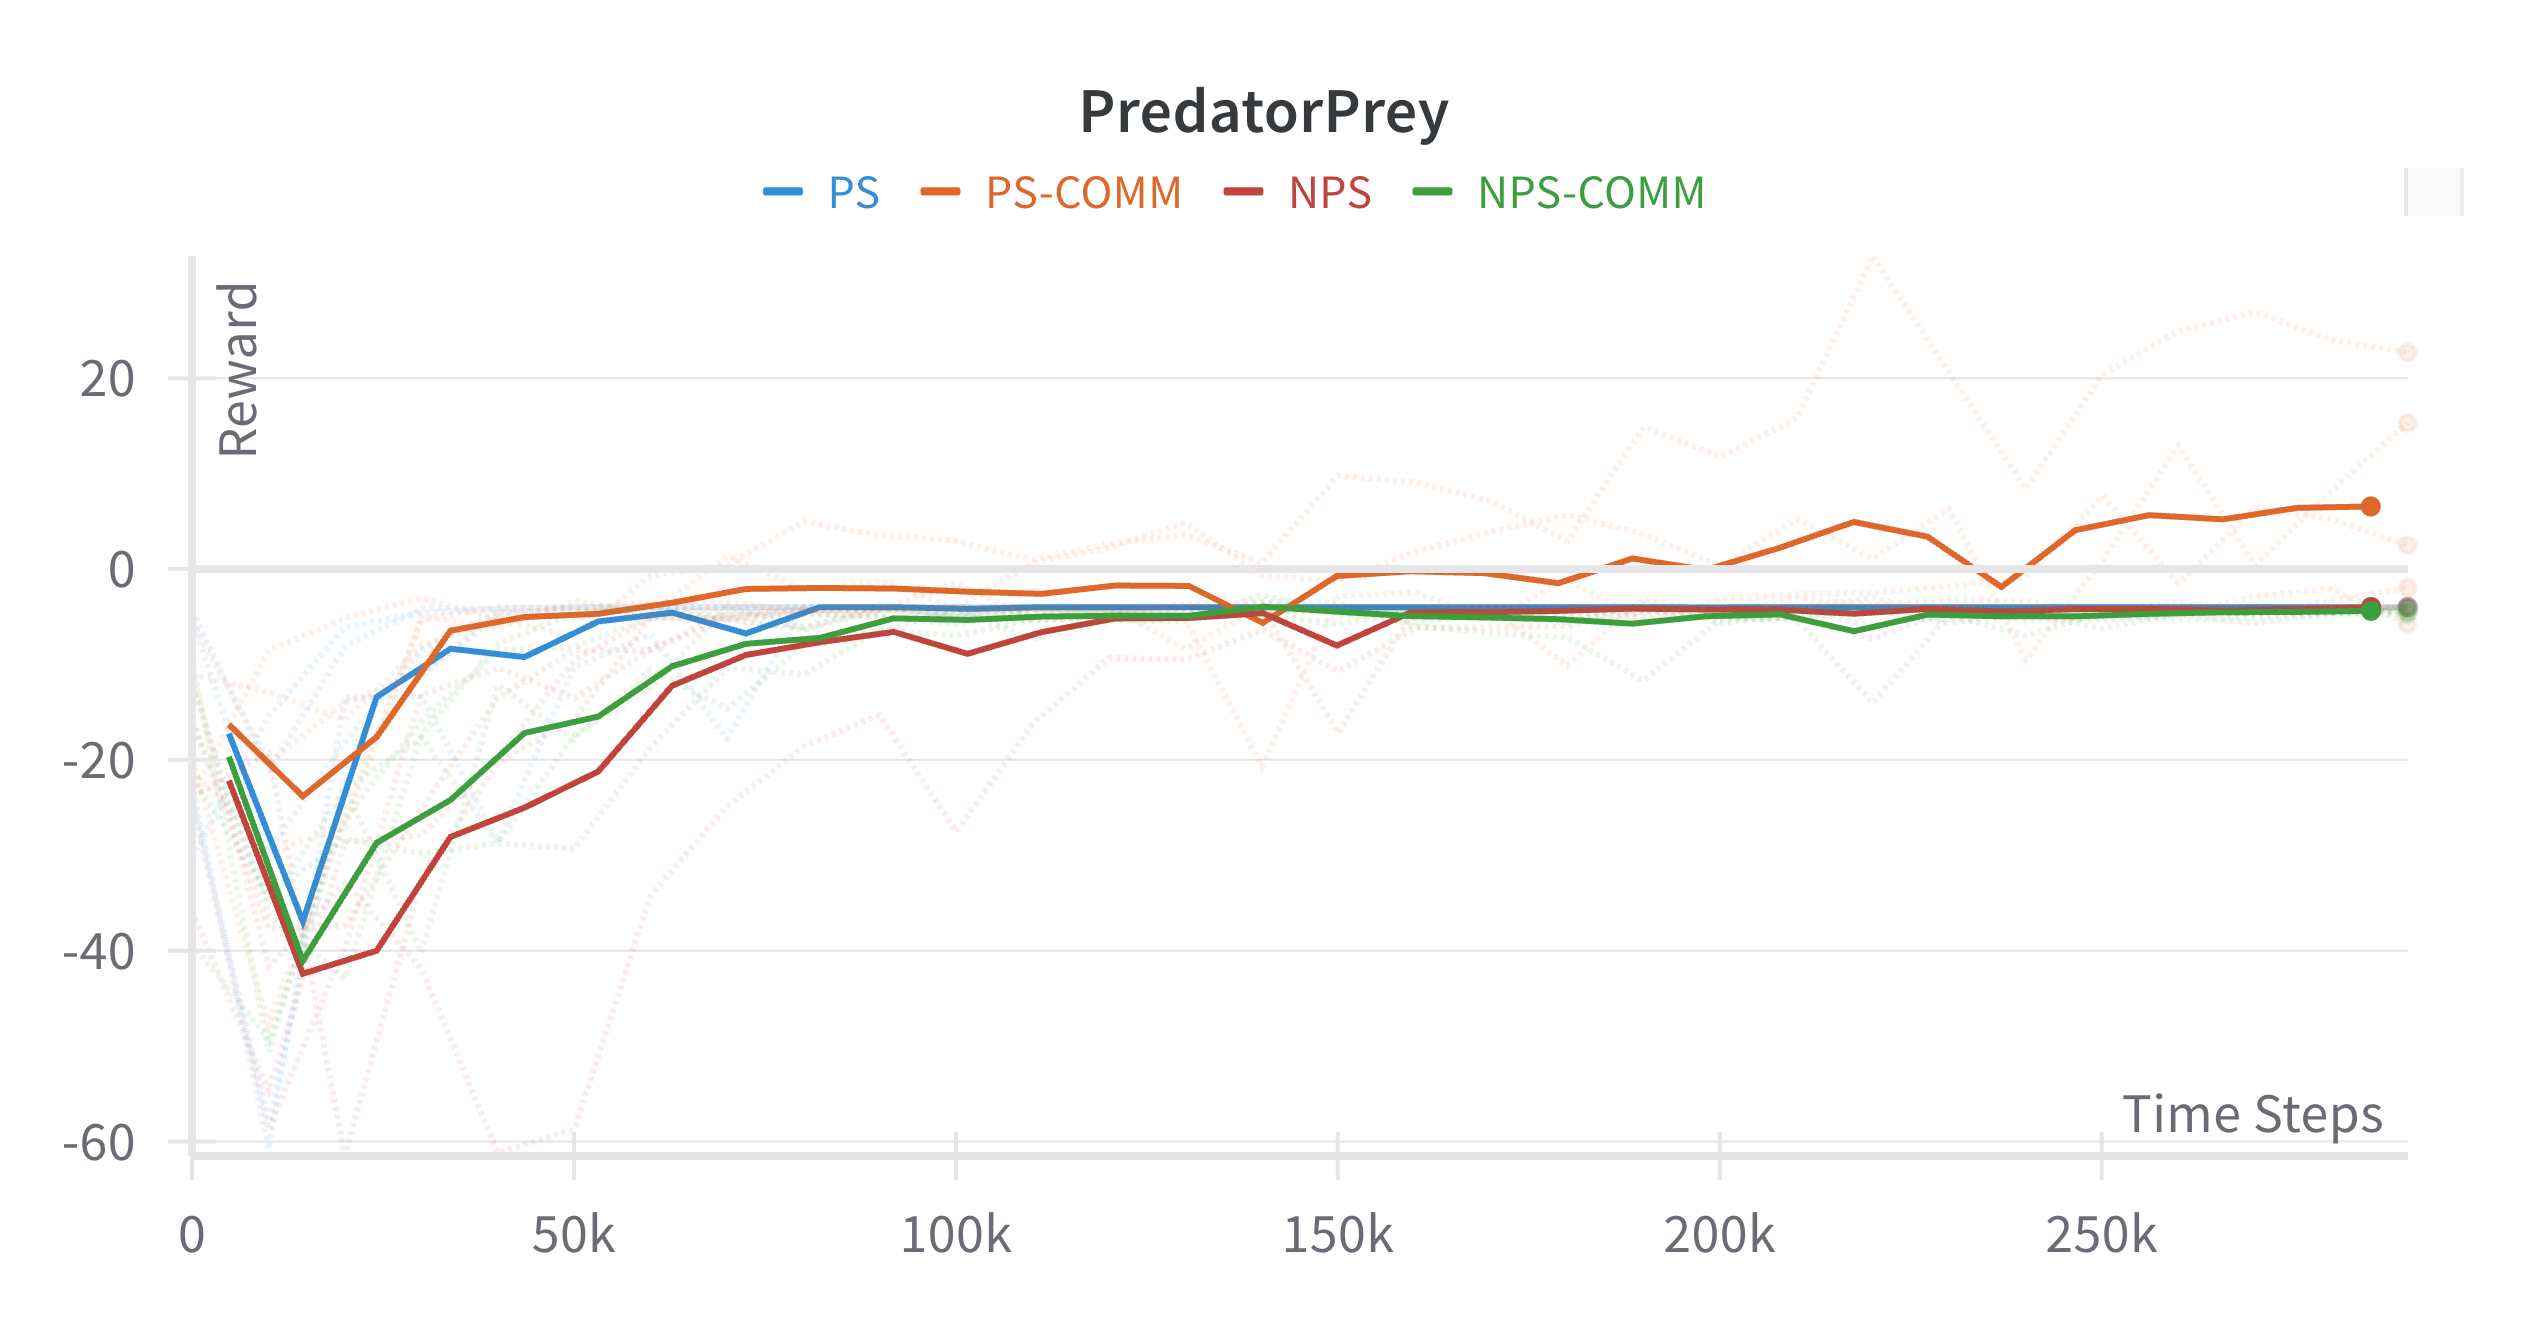
\includegraphics[width=\textwidth]{images/PredatorPreyResults.png}
        \caption{Predator-Prey Results}
        \label{fig:predator_prey_results}
    \end{subfigure}
    \hfill
    \begin{subfigure}[b]{0.9\textwidth}
        \centering
        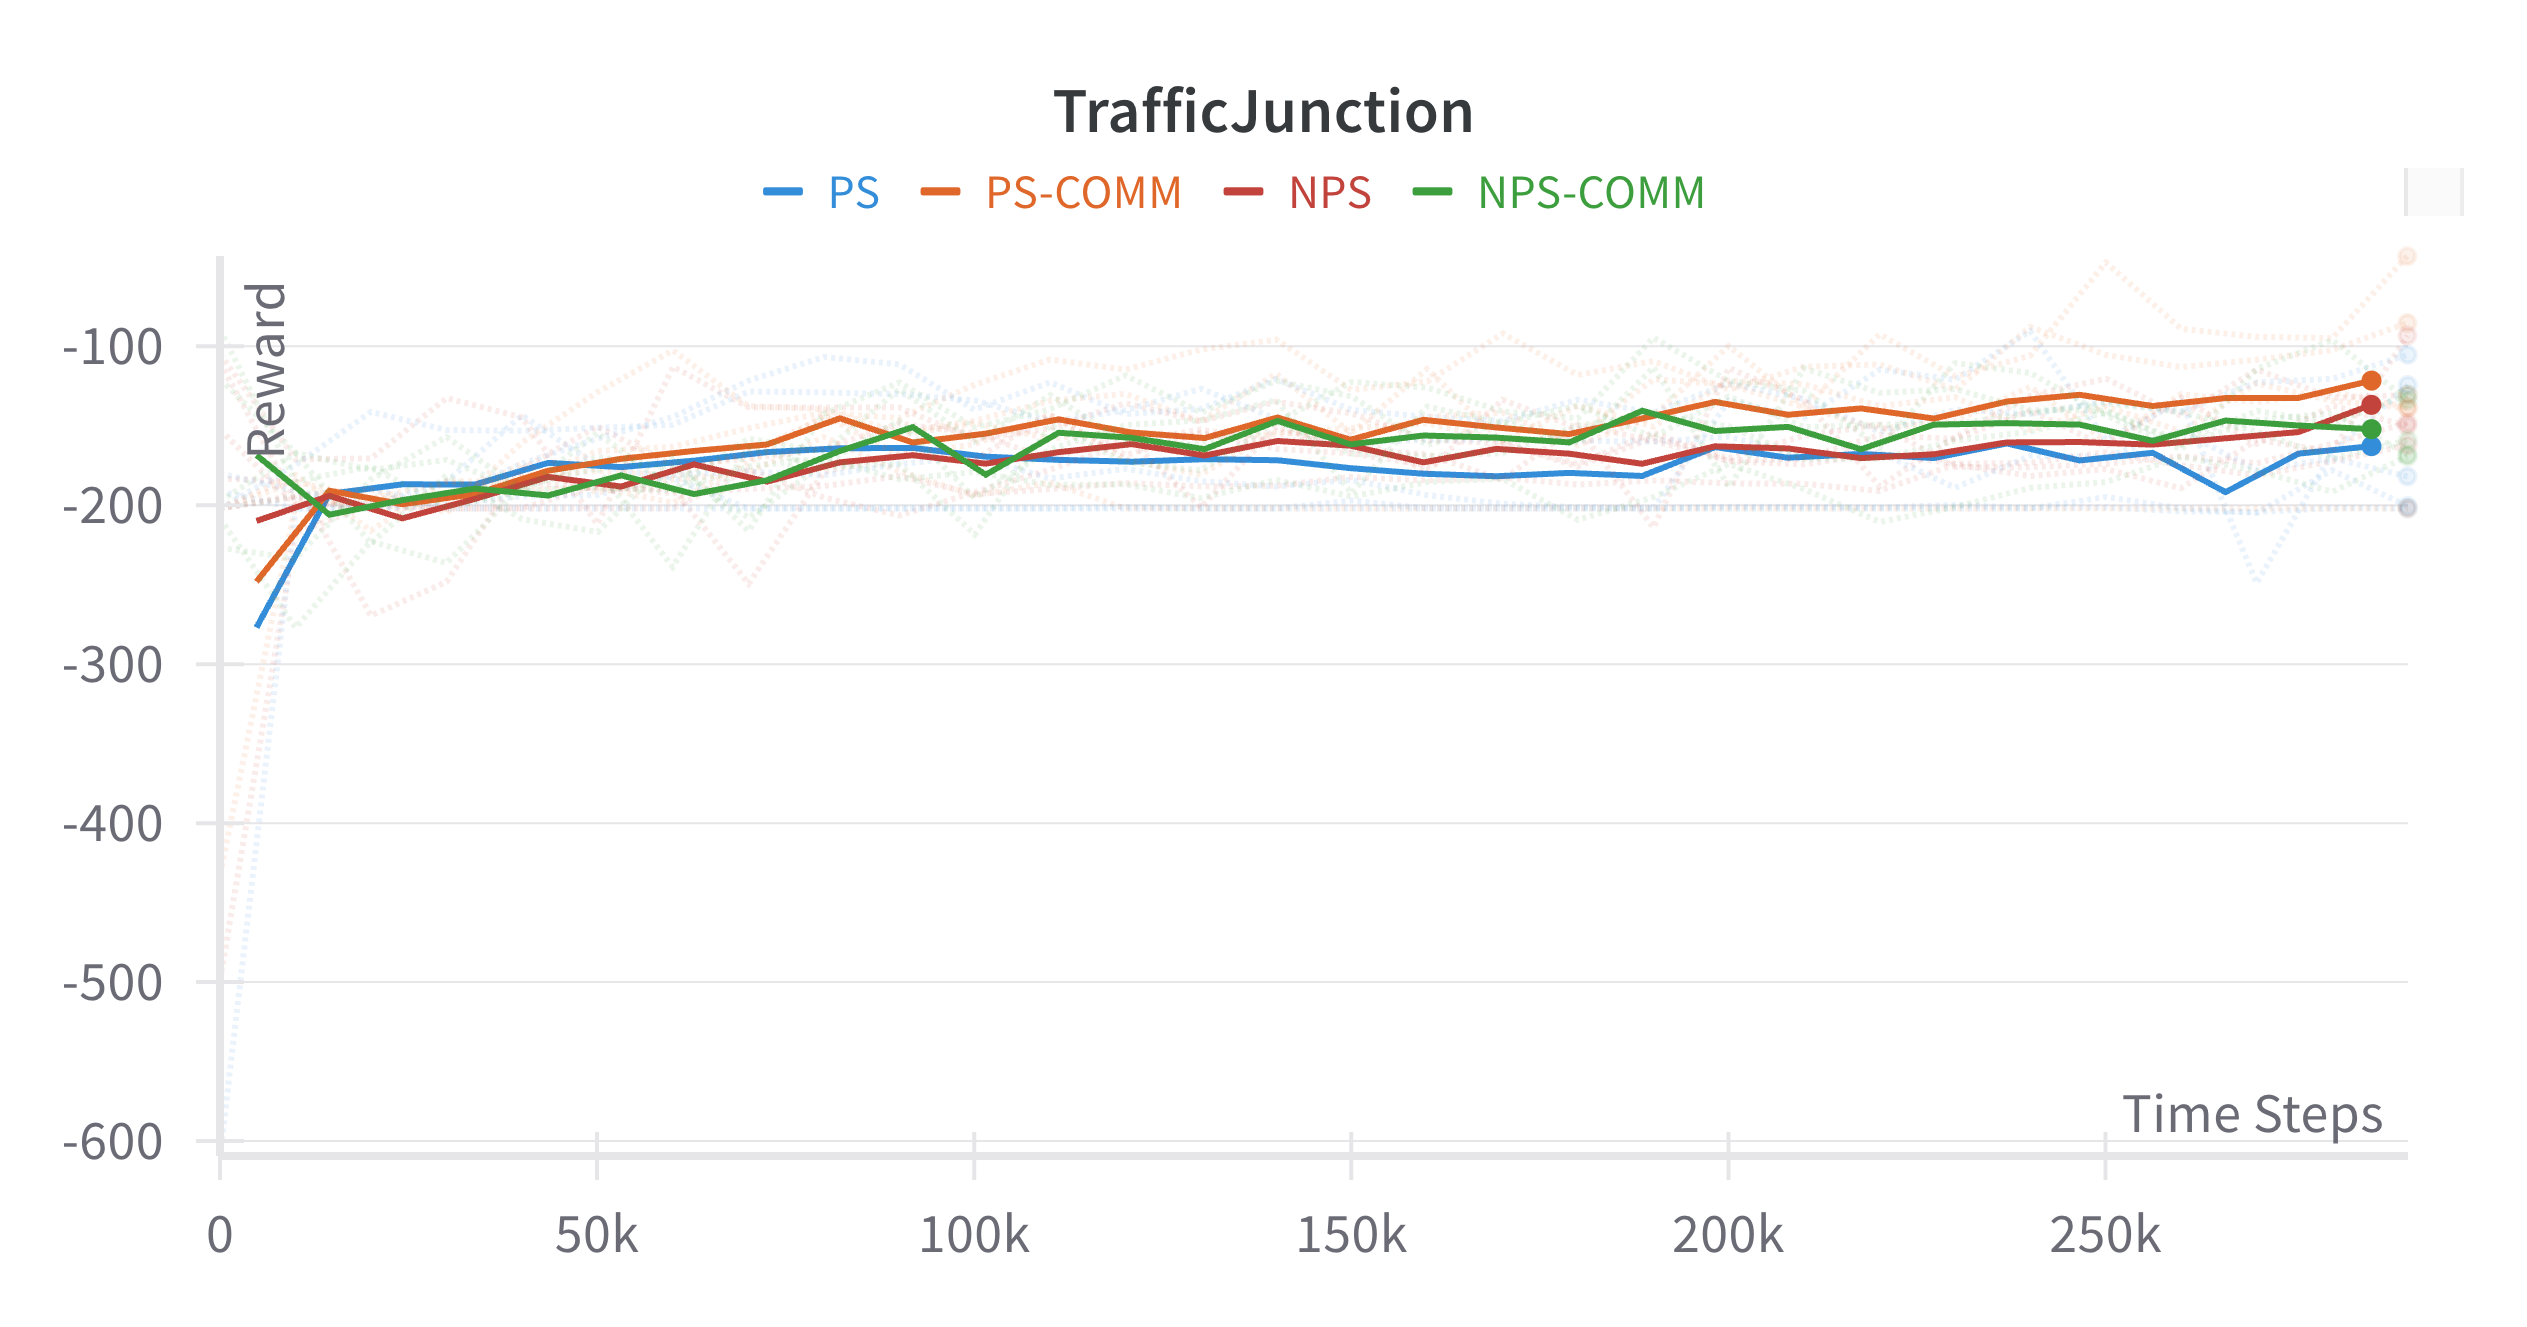
\includegraphics[width=\textwidth]{images/TrafficJunctionResults}
        \caption{Traffic Junction Results}
        \label{fig:traffic_junction_results}
    \end{subfigure}
    \caption{Results from the experiment in the Predator-Prey environment and the Traffic Junction. The four treatments: PS, PS-COMM, NPS, NPS-COMM were run five times in each environment for 300k time-steps with the average across the trails plotted. In (\ref{fig:predator_prey_results}) we observe the only model that has improved performance if the PS-COMM model. While in (\ref{fig:traffic_junction_results}), all models performed very similarly.}
    \label{fig:results}
\end{figure}

In the Predator-Pray environment, we observe that the PS-COMM model was able to outperform all other models. This is consistent with the results from \citet{pina2024fully}. However, in their investigation they found that a hidden layer size of 128 for the NPS-COMM was able to outperform the other two models, with results comparable to that of PS-COMM. While in this investigation all model's a hidden dimension of 128. This was due to issues with computation time. The learning curves for PS, NPS and NPS-COMM are very similar with rewards plateauing at around the 75k time step. Again this is a result consistent with \citet{pina2024fully} when using 64 dimensions in the hidden layer. 

\

In the Traffic Junction environment, we observe no significant difference between the performance of any of the models. This is most likely due to the lack of parameter tuning within the environment; since all the the same neural network hyper-parameters were used from the Predator-Pray, the model is likely in the wrong region of the parameter space. Despite this, learning does seem to be occurring within the models as we observe a consistent upward gradient in the average reward line plotted.

\

It is encouraging to see comparable performance between the PS and NPS-COMM model, given that parameter sharing has been such a fundamental assumption in many MARL algorithms. However, issue with the NPS models is that of computation and learning time. Since we are storing a policy and messaging neural network for each agent, in an environment with 4 agents, the number of neural networks to store increases to 8 which meant that the NPS-COMM model took over double the time (25 minutes) compared to the PS model (12 minutes) on average to complete the 300k time steps. While this is an issue since the computations were all running on one machine, when scaling this to multiple agents each capable of computation, it is easy to see how this is no longer a problem.

\clearpage

\section{Conclusion}

In this report, we began by establishing a foundation in RL, building from fundamental concepts such as MDPs, q-learning, and policy-based methods to deep reinforcement learning techniques. This foundation provided a crucial framework to explore the unique challenges of MARL, where multiple autonomous agents interact within a shared environment. Key issues in this context include non-stationarity - arising from each agent's evolving policy that renders the environment dynamics unstable - and the problem of credit assignment, where it becomes challenging to attribute success or failure to individual agents' actions within a collective system.

\

To address these issues, we introduced the concept of communication, drawing motivation from human approaches to collaboration and coordination in complex environments. Effective communication allows agents to share crucial information, potentially stabilising learning dynamics and enhancing each agent's understanding of the environment and of other agent' intentions. We explored the importance of communication in multi-agent reinforcement learning (MARL) through a detailed review of the literature, identifying critical dimensions that help us classify and analyse the spectrum of Comm-MARL models. Using the nine dimensions proposed by \citet{zhu2024survey}, we provided a structured approach to understanding this evolving field. These dimensions capture aspects of problem setting, communication processes and training processes.

\

An essential point arising from this review is the role of parameter sharing as a fundamental assumption across many Comm-MARL models. Parameter sharing is often implemented either with or without an agent-specific indicator, allowing agents to generalise their learned policies while still enabling specialised behaviours. This assumption simplifies the model architecture and has been shown to improve learning stability and efficiency. However, it also raises questions about the trade-offs between model simplicity and the flexibility to allow agents to develop different strategies.

\

The empirical study in the final section of this report tested these concepts through an investigation into four model variations based on the architecture introduced by \citet{pina2024fully}. These models, differing in their use of parameter sharing and communication, were evaluated within two distinct environments: the Predator-Prey environment and the Traffic Junction environment. These settings provided controlled, yet complex, tasks that helped to illustrate the impact of communication and parameter sharing on learning outcomes in multi-agent systems.

\

Results indicate that the model utilising both parameter sharing and communication showed the greatest improvement in performance in the Predator-Prey environment, highlighting the benefits of a shared parameter space combined with inter-agent message exchange in scenarios requiring close cooperation and coordination. Interestingly, the model with communication but without parameter sharing demonstrated comparable performance, suggesting that communication alone may enable effective collaboration without necessitating identical parameter spaces across agents. This finding points to the potential of communication as a powerful mechanism for scaling and distributing MARL systems, especially in scenarios where parameter sharing may be infeasible or undesirable.

\

In conclusion, this study motivates the value of communication in multi-agent settings and suggests promising avenues for further exploration. By leveraging communication, MARL systems can achieve scalable and robust performance, even in complex and dynamic environments, paving the way for broader applications in areas such as autonomous driving, collaborative robotics, and distributed AI.

\newpage

\bibliography{references}
\addcontentsline{toc}{section}{References}

\newpage

\appendix

\section{Supplementary Material}
All code for the experiment and plot generation can be found at: \url{https://github.com/jackbmontgomery/comm-marl}


\section{MARL Communication Models} \label{sec:models}
\subsection{RIAL and DIAL}\label{subsec:dial_rial}

Both \textbf{r}einforced \textbf{i}nter-\textbf{a}gent learning (RIAL) and \textbf{D}ifferentiable \textbf{i}nter-\textbf{a}gent learning (DIAL) were proposed in \citet{foerster2016learning}. These models are architecturally identical but are differentiated by the way the gradients of the parameters responsible for generating messages are computed during learning.

\

The foundations for this model are in deep q-networks, deep recurrent q-networks and independent q-learning. A key difference is the disabling of experience replay in the RIAL and DIAL models because the non-stationarity of the multi-agent environment caused the agent to learn from obsolete and misleading data. The specific training and execution configuration considered in these models is one of centralised training and decentralising execution. Moreover, only discrete messages are considered in these models. 


\paragraph{RIAL} Each agent's q-network is represented by $Q^a(o_t^a, m_{t-1}^{a'}, h_{t-1}^{a}, u^a)$ which are all conditioned on the agent indexed by $a$, where $a'$ refers to the other agents. To avoid a network with output dimension $|U||M|$, the q-network is split between the environment ($Q^a_u$) and communication ($Q^a_m$) action networks. There is then an actor selector that picks $u_t^a$ and $m_t^a$ from the Q-value output using an $\varepsilon$-greedy policy. Hence, the network requires only $|U| + |M|$ outputs and action selection requires maximising over U and then over M , but not maximising over $|U| \times |M|$.

\paragraph{Parameter Sharing} RIAL can be extended to take advantage of the opportunity for centralised learning by sharing parameters among the agents. This variation learns only one network, which is used by all agents. However, the agents can still behave differently because they receive different observations and thus evolve different hidden states. In addition, each agent receives its own index a as input, allowing them to specialise.

\paragraph{DIAL} While RIAL can share parameters among agents, it still does not take full advantage of centralised learning. In particular, the agents do not give each other feedback about their communication actions. Contrast this with human communication, which is rich with tight feedback loops. The main insight behind DIAL is that the combination of centralised learning and q-networks makes it possible, not only to share parameters but to push gradients from one agent to another through the communication channel. DIAL achieves this with the use of the C-net (Communication network) instead of the q-network. The C-network also outputs communication vectors, as well as action vectors from local observations. This adjustment, along with the parameter sharing between agents' networks, let gradients flow from one agent to another. This enables a richer feedback loop, reducing the required amount of learning by trial and error, and easing the discovery of effective protocols. The end-to-end differentiability is disrupted with the discrete nature of the messages. To navigate this, \citet{foerster2016learning} propose the DRU (discretise and regularise unit) for messages to pass through before being received by other agents. The DRU has separate functions during training and execution. In training, the DRU is tasked with encouraging the agents to learn protocols that can be easily discretised. This is done by passing the message through a sigmoid activation function and adds noise. Then, during execution, the messages are discretized by the DRU: $DRU(m_t^a) = 1\chi_{\{ m_t^a > 0 \}}$, where $\chi$ is the indicator function.

\

\begin{figure}
	\centering
	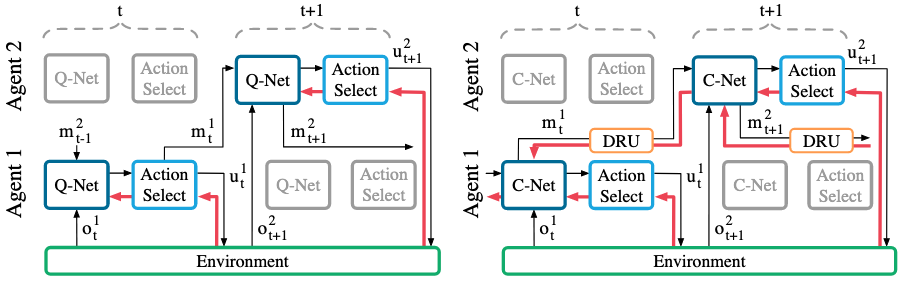
\includegraphics[scale=0.5]{images/rial_dial.png}
	\caption{Image from \citet{foerster2016learning} depicting the RIAL and DIAL model architectures, with inputs and messages shown by black arrows and gradients shown by red arrows. (Left) RIAL model where gradients are computed with respect to the feedback from the environment. (Right) DIAL model using the DRU that all messages pass through, as well as the direct gradient sharing between agents which uses parameter sharing.}
\end{figure}

The architecture used in both RIAL and DIAL models is identical. As illustrated in Figure \ref{fig:rial_dial_nn}, each agent is composed of a RNN, unrolled over \( T \) time-steps, which maintains an internal state \( h \). This architecture includes an input network for generating a task embedding \( z \), as well as an output network for producing Q-values and messages \( m \). The input for agent \( a \) is specified as a tuple \( (\mathbf{o}_t^a, m_{t-1}^{a'}, u_{t-1}^a, a) \). Here, the components \( a \) and \( u_{t-1}^a \) are processed through lookup tables, while \( m_{t-1}^{a'} \) is processed via a 1-layer MLP, each generating embeddings of size 128. The observation \( \mathbf{o}_t^a \) is passed through a task-specific network that generates an additional embedding of the same size. The final state embedding is then produced by the element-wise summation of these embeddings:

$$
\mathbf{z}_t^a = (\text{TaskMLP}(\mathbf{o}_t^a) + \text{MLP}[|M|, 128](m_{t-1}) + \text{Lookup}(u_{t-1}^a) + \text{Lookup}(a)).
$$

The original authors observed improved performance and stability when batch normalisation \citep{ioffe2015batch} was applied to \( m_{t-1} \) before processing. The combined embedding \( \mathbf{z}_t^a \) is subsequently processed through a 2-layer RNN with GRUs:

$$
h_{1, t}^a = \text{GRU}[128, 128](\mathbf{z}_t^a, h_{1, t-1}^a),
$$

serving as an approximation of the agent’s action-observation history. Finally, the output \( h_{2, t}^a \) from the top GRU layer is fed into a 2-layer MLP to produce both the Q-values and the message:

$$
\mathbf{Q}_t^a, \mathbf{m}_t^a = \text{MLP}[128, 128, (|U| + |M|)](h_{2, t}^a).
$$


\begin{figure}
	\centering
	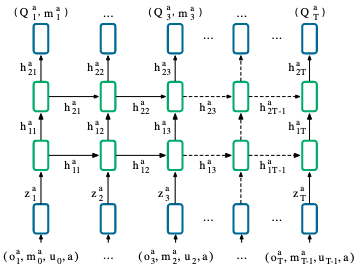
\includegraphics[scale=0.7]{images/rial_dial_nn.png}\
	\caption{Architecture of the RIAL and DIAL models from \citet{foerster2016learning}. Each agent comprises a recurrent neural network (RNN) unrolled over \( T \) time-steps, which maintains an internal state \( h \). Inputs, including observations \( \mathbf{o}_t^a \), previous messages \( m_{t-1}^{a'} \), previous actions \( u_{t-1}^a \), and agent identity \( a \), are embedded and combined to produce a state embedding \( \mathbf{z}_t^a \). The embedding is processed through a 2-layer RNN with GRUs to approximate the agent’s action-observation history. The output is then passed through a 2-layer MLP to generate both the Q-values and the message \( \mathbf{m}_t^a \).}
	\label{fig:rial_dial_nn}
\end{figure}

\subsection{CommNet}

\citet{sukhbaatar2016commnet} propose the communication neural network (CommNet) model which is centred around the global controller, $\Phi$, used for the computation of the actions and messages. Unlike, \citet{foerster2016learning} these messages are continuous vectors. The controller maps the concatenation of all local observations at a point in time, $\mathbf{o} = \{ o_1, \hdots, o_J \}$\footnote{Time index is omitted for brevity}, to the concatenation of all actions, $\mathbf{a} = \{ a_1, \hdots, a_J \}$, for $J$ agents. Thus, $\mathbf{a} = \Phi(\mathbf{o})$. 

\

The structure of the controller is of the form of a neural network comprised of modules, $f^i$, for each communication step $i$. The modules take as input the hidden state $h^i_j$ and the communication $c^i_j$,  and outputs a vector $h^{i+1}_j$. The main body of the model then takes as input the concatenated vectors $\mathbf{h}^i = [h^i_1, \hdots,  h^i_J]$, and computes:


\begin{equation}\label{eq:commnet_equations}
\begin{aligned}
	h_j^{i+1} &= f^i(h^i_j, c^i_j) \\
	c_j^{i+1} &= \frac{1}{1 - J} \sum_{j' \neq j} h_{j'}^{i + 1}
\end{aligned}
\end{equation}

$f^i$ is a single layer neural network with a sigmoid non-linearity $\sigma$. In which case, $f^i(h^i_j, c^i_j) = \sigma(H^i h^i_j +  C^i c^i_j)$. The use of the normalisation for the messages is due to the fact that the number of agents can increase, in such a case we then rescale the communication vector.

\

At the first layer of the model an encoder function $h_j^0 = r(s_j)$ is used. This takes as input the local observation $o_j$ and outputs feature vector $h_j^0$ (in $R_{d_0}$ for some $d_0$). The form of the encoder is problem dependent,  but for most of our tasks it is a single layer neural network with $c_j^0 = 0$ for all $j$.  

\

Each layer of the model corresponds to a communication step in the language of the paper. In these layers the computations highlighted in (\ref{eq:commnet_equations}) where the new hidden layers, and messages there after are computed.

\

At the output of the model, a decoder function $q(h_j^K)$ is used to output a distribution over the space of  actions. $q(\cdot)$ takes the form of a single layer network, followed by a softmax. To produce a discrete  action, we sample from this distribution: $a_j \sim q(h_j^K )$.  

\begin{figure}
	\centering
	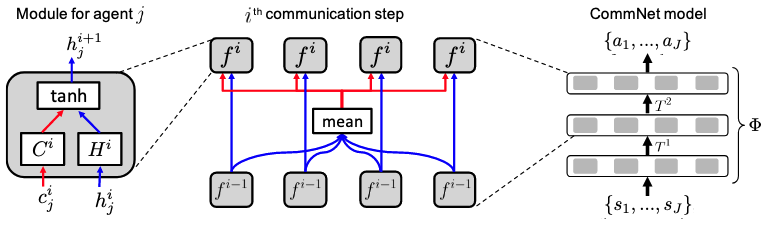
\includegraphics[scale=0.5]{images/commnet.png}
	\caption{Architecture of the central controller of CommNet \citep{sukhbaatar2016commnet}}
	\label{fig:commnet}
\end{figure}

\

Modifications and extension were proposed to the model. These include:
\begin{itemize}
	\item Local connectivity where the message communication is computed based on the value of local hidden states. In which case, a network of agent's are formed and the passing of the aggregated hidden states corresponds to Belief Propagation. \citep{pearl1982bayes}
	\item Skipping connections where the first input encoding $h_0^j$ is present for inputs beyond the next communication step.
	\item Temporal recurrence where a connection between the modules is created between time-steps. In which case the final hidden states is fed as input into the initial input encoding in the next time-step. 
\end{itemize}

\subsection{IC3Net}

Individualised Controlled Continuous Communication Model (IC3Net) is a model proposed by \citet{singh2018ic3net} and represents an extension to the CommNet model \citep{sukhbaatar2016commnet}. The model's extension's are centred around a gating mechanism for the messages that the agent communicate. This allows agent's to not only learn to communicate, but learn when to communicate. As such, then mechanism allows the CommNet \citep{sukhbaatar2016commnet} to be extended to mixed and cooperative environments. 

\begin{figure}
	\centering
	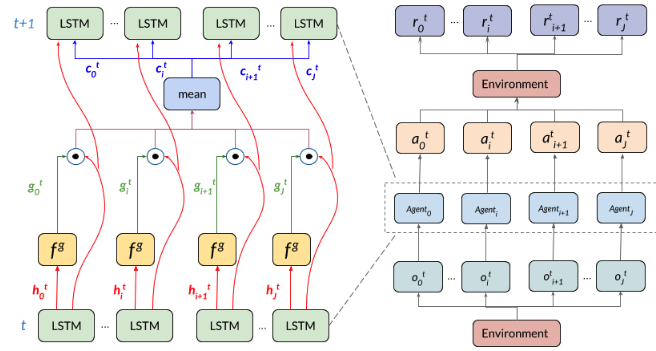
\includegraphics[scale=0.5]{images/ic3net.png}
	\caption{Architecture of IC3Net \citep{singh2018ic3net}. \textbf{Left}: Depicts the computational dependencies between the components of the model that an agent possess for a single communication step. \textbf{Right:} Depicts the relationship between the objects in the environment and the agents.}
	\label{fig:ic3net.png}
\end{figure}

\

IC3Net is based on an independent controller model where each agent is controlled by an individual LSTM \citep{hochreiter1997long}. For the $j-th$ agent, its policy takes the form of:

\begin{equation}
	\begin{aligned}
		h_j^{t + 1} &= LSTM(e(o_j^t), h_j^t, s_j^t) \\
		a^t_j &= \pi(h^t_j)
	\end{aligned}
\end{equation}

where $o_j^t$ is the observation of the $j-th$ agent at time $t$, $e(\cdot)$ is an encoder function parameterised by a fully-connected neural network and $\pi$ is an agent’s action policy, $h^t_j$ and $s^t_j$ are the hidden and cell states of the LSTM. The same LSTM model is used for all agents, therefore engaging in parameter sharing. This way, the model is invariant to permutations of the agents. \citep{singh2018ic3net}

\

IC3Net extends the independent controller model by allowing agents to communicate their internals states, gated by discrete action. The policy of the $j-th$ agent is given by:

\begin{align*}
    g_j^{t+1} &= f^g\left(h_j^t\right) \\
    h_j^{t+1}, s_j^{t+1} &= \text{LSTM}\left(e\left(o_j^t\right) + c_j^t, h_j^t, s_j^t\right) \\
    c_j^{t+1} &= \frac{1}{J-1} C \sum_{j' \neq j} h_{j'}^{t+1} \odot g_{j'}^{t+1} \\
    a_j^t &= \pi\left(h_j^t\right)
\end{align*}

where $c^t_j$ is the communication vector for the $j-th$ agent, $C$ is a linear transformation matrix for transforming gated average hidden state to a communication tensor, $J$ is the number of alive agents currently present in the system and $f^g(\cdot)$ is a simple network containing a soft-max layer for 2 actions (communicate or not) on top of a linear layer with non-linearity. The binary action $g^t_j$ specifies whether agent $j$ wants to communicate with others, and act as a gating function when calculating the communication vector. Note that the gating action for next time-step is calculated at current time-step. The action policy $\pi$ and the gating function $f^g$ with REINFORCE \cite{williams1992simple}.

\

In Commnet \citep{sukhbaatar2016commnet} individual networks controlling agents were interconnected, and they as a whole were considered as a single, large neural network. This single network controller approach required a definition of a unified loss function during training, thus making it impossible to train agents with different rewards. 

\

IC3Net \citep{singh2018ic3net} moves away from the single big network controller approach. Instead, it uses multiple large networks with shared parameters each controlling a single agent separately. Each big network consists of multiple LSTM networks, each processing an observation of a single agent. However, only one of the LSTMs needs to output an action because the big network is only controlling a single agent. Although this view has a little effect on the implementation - since a single neural network was still used in practice - it allows them to train each agent to maximise their individual reward instead of a single global reward. This has two benefits: firstly, it allows the model to be applied to both cooperative and competitive scenarios, secondly, it also helps resolve the credit assignment issue faced by many multi-agent algorithms. 

\subsection{BiCNet}

Multi-agent Bidirectionally-Coordinated Net (BiCNet) \citep{peng2017bicnet} is a model that leverages a bidirectional Recurrent Neural Network (bi-RNN) \citep{chuster1997Bidirectional} to facilitate the communication. While learning is done using a multi-agent actor-critic framework. Further, BiCNet \citep{peng2017bicnet} leverages parameter sharing in order to solve scalability issues with respect to increasing the number of agent.

\

\begin{figure}
	\centering
	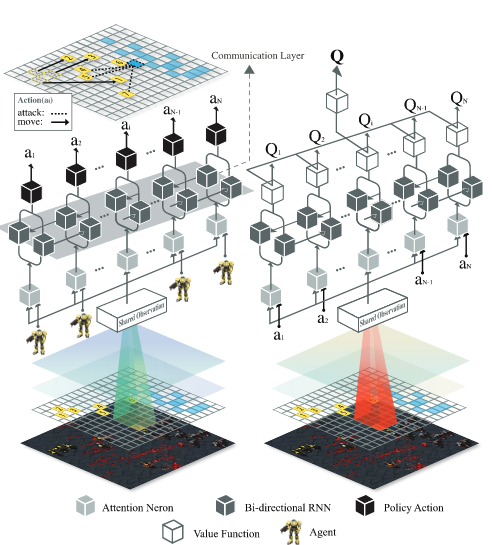
\includegraphics[scale=0.5]{images/bicnet}
	\caption{Architecture of the actor network (Left) and critic network (Right) for BiCNet \citep{peng2017bicnet}}
	\label{fig:ic3net.png}
\end{figure}

BiCNet shares parameters across agents to ensure that the model is compact and scalable, allowing it to handle varying numbers of agents without needing retraining. This parameter-sharing mechanism is similar to RNNs, where parameters are shared across time steps. Each agent’s internal state and observed information are shared bidirectionally with other agents, promoting effective communication. By using bi-RNNs, BiCNet is not restricted to symmetric communication, enabling roles and priorities among agents, which aids in collaborative strategies.

\

Training employs backpropagation through time \citep{werbos1990backpropagation} over the bi-RNN structure, calculating gradients jointly across the actor and critic networks. Specifically:

\begin{itemize}
    \item \textbf{Actor Gradient:} A multi-agent deterministic policy gradient is applied to optimise the actor, where each agent’s policy is collectively learned across agents, leading to aggregate reward optimisation.
    
    \item \textbf{Critic Gradient:} A squared loss gradient is used to optimise the critic network, where each agent’s Q-values are evaluated based on the reward and expected future reward.
    
    \item \textbf{Experience Replay:} The model uses experience replay to stabilise training, storing past interactions and sampling mini-batches to train the networks iteratively. This replay allows the agents to learn effectively from past experience rather than only recent events.
    
    \item \textbf{Exploration with Ornstein-Uhlenbeck Process:} To add stochasticity during training, the model applies noise to the actor's actions, facilitating better exploration, especially in continuous action spaces.
\end{itemize}

\textbf{Message Encoding through Hidden States:} In BiCNet, communication occurs through hidden states passed between agents in the bi-RNN layers. In other words, this communication is done in the latent space. This process allows each agent to integrate information from others and decide actions based on both local states and shared communication, while not conditioning their actions directly on the actions of other agents meaning that high-level information can be passed between agents \citep{peng2017bicnet}.

\subsection{NeurComm}

NeurComm \citep{chu2020NeurComm} is a model that positions itself within the subfield of networked multi-agent reinforcement learning (NMARL). Which is a paradigm of MARL that assumes communication channels between local connected neighbours. These connections then form the network of agents ($\mathcal{N}_i$ will denote the neighbourhood of agent $i$). NeurComm \citep{chu2020NeurComm}  exploits the spatiotemporal dimension of this network. The Markov property is then assumed to be present in both the spatial and temporal dimensions. 

\
 To illustrate the messaging protocol let us assume all messages sent from agent $i$ in this model are assumed to be equal: $m_{ij} = m_i, \ \forall j \in \mathcal{N}_i$. Then:

\begin{equation}
	h_{i, t} = g_{\nu_i} (h_{i, t-1}, e_{\lambda_i^s}(s_{\mathcal{V}_i, t}), e_{\lambda_i^p}(\pi_{\mathcal{N}_i, t-1}), e_{\lambda_i^h}(h_{\mathcal{N}_i, t-1}))
\end{equation}

Where $h_{i, t}$ is the hidden state of agent $i$ at time $t$. $e_{\lambda_i}$ and $g_{\nu_i}$ are differentiable message encoding and extracting functions. To avoid dilution of state and policy information (the former is for improving observability while the later is for reducing non-stationarity), state and policy are explicitly included in the message besides agent belief. This means:

\begin{equation}
	m_{i,t} = s_{i,t} \cup \pi_{i,t−1} \cup h_{i,t−1}
\end{equation}

The communication phase is prior-decision, so only $h_{i,t−1}$ and $\pi_{i,t−1}$ are available. Described is a single pass of communication, but it can easily be extended to multiple passes. 

\

NeurComm can be represented using a single meta deep neural network  since all agents are connected by differentiable communication links, and $\tilde{s}_i$ are the intermediate outputs after communication layers. Figure \ref{fig:neurcomm} (Left) illustrates the forward propagations inside each individual agent and \ref{fig:neurcomm} (Right) shows the broader multi-step spatiotemporal propagations. The gradient propagation of this meta-DNN is decentralised based on each local loss signal. As time advances, the involved parameters in each propagation expand spatially in the meta-DNN, due to the cascaded neighbourhood communication.

\begin{figure}
	\centering
	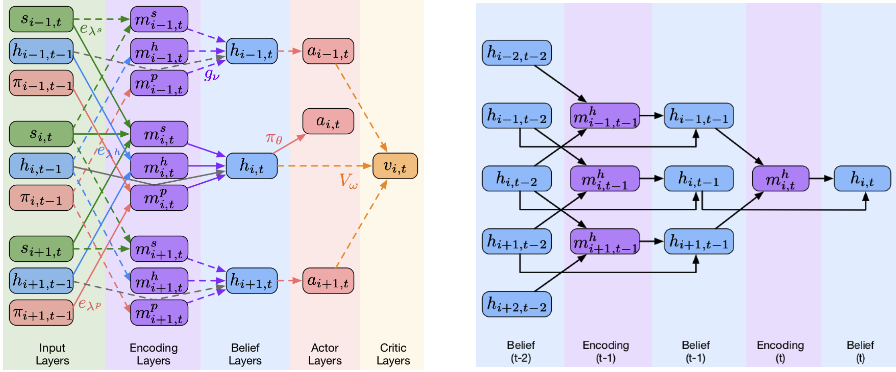
\includegraphics[scale=0.5]{images/neurcomm}
	\caption{Neural network architecture of \citet{chu2020NeurComm} showing forward propagations illustrated in a queueing system. (Left): Single-step forward propagations inside agent $i$. Different coloured boxes and arrows show different outputs and functions, respectively. Solid and dashed arrows indicate actor and critic propagations, respectively. (Right): Multi-step forward propagations for updating the belief of agent $i$.}
	\label{fig:neurcomm}
\end{figure}

\subsection{HAMMER}

The Heterogeneous Agents Mastering Messaging to Enhance Reinforcement learning (HAMMER) \citep{gupta2022HAMMER} presents an architecture based on local learners and a central learner. The local learners are the agents performing actions in the environment, while the central learner serves as a proxy for generating messages that aid coordination among these agents. 

\

At the start of each time step, the central agent receives the observations of all agents, denoted as $\mathbf{o^t} = [o_1^t, \hdots, o_j^t]$, where $o_j^t$ represents the observation of agent $j$ at time $t$. The central agent processes this combined observation and outputs a personalised message $m_i^t$ for each agent $i$. These messages represent the actions that the central learner is able to take at each time step. Each independent agent then combines its local observation $o_i^t$ with the received message $m_i^t$ to inform its action selection within the environment. The agent then receives its reward feedback from the environment. These dynamics are illustrated in Figure \ref{fig:hammer}.

\begin{figure}
	\centering
	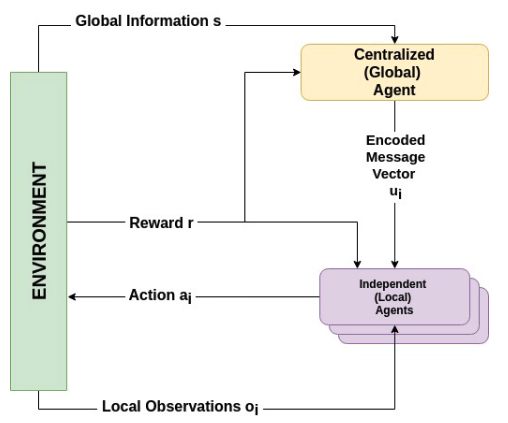
\includegraphics[scale=0.5]{images/hammer}
	\caption{Image from \citet{gupta2022HAMMER} depicting the information exchange of the HAMMER model during a single time-step.}
	\label{fig:hammer}
\end{figure}

\

The independent agents implement Proximal Policy Optimisation (PPO) \citep{schulman2017proximal} as their reinforcement learning model. To ensure consistent policy updates and computational efficiency, the local agents use parameter sharing, where a single network with shared parameters represents the policies of all agents. This shared network structure enables experience collected by each agent to contribute toward updating a common policy. During learning, the agent is constructing a policy based on the input from the local observation, as well as the messages it receives which enables the agent to learn to potentially ignore the messages if the gradients determine the content of the message is not useful for actions within the environment. 

\

The central agent learning is implemented in two different ways:
\begin{enumerate}
    \item The agent can learn from the rewards received by local agents as the gradient signal
    \item Gradients computed by the local agent's during learning - that is done by connecting the output of the central agent's network to the input of the local agents policy network
\end{enumerate}

These two learning paradigms represent a reinforced vs a differentiable approach to learning the communication protocol, similar to the distinction between RIAL and DIAL in \citet{foerster2016learning}. What's more, the third implementation of HAMMER assumes a DRU to enable discretised communication during execution, while maintaining the differentiability of the neural networks during training.

\

HAMMER employs experience replay with two separate memory buffers: one for the local agents and one for the central agent. The replay buffers store experiences, allowing the central and local agents to sample past interactions during updates. This approach enhances sample efficiency and reduces variance in the learning process.

\end{document}






























